% STATUS: ACTIVE -- c-only slope law (p = 2): the Q/R-ratio design of the c slot (Q55 = R_k rho_k), definitions, the P_0 scan,
%   the opponents (constant rho, literal R2 ratio), speed, the oscillation trajectories and the innovation gate (2026-09-30 .. 10-02).
%   Ledger: hypotheses_formC_b.md C82-C85, R70-R74, O47-O51. Memory: project_q55_ratio_design_2026-10-02.
% ======================================================
% Compile: xelatex 0930_q55_ratio_design.tex   (from reference/eq17_analysis/derivation/)
% Format: 0928_obs_c_only_v1.tex (same preamble, same SSOT notation, equations only; headings are the one-line definitions).
% Code: motion_control_law_formC_b.m, ctrl_const.q55_adapt = 'ratio' (q55_adapt_P0 = sqrt(P_0), 0 = the slot-5 prior) | 'rhoconst' (q55_adapt_rho,
%   q55_adapt_Imin) | 'r2ratio' (q55_adapt_rho) | 'ratiogate' (q55_adapt_N, q55_adapt_thr); q55_adapt_hgate (height gate, Inf = off); all default off.
%   Trajectories: trajectory_type 'osc_linear' (= 0, constant-velocity descent) and 'osc_tri' (= -1, triangle), default 'osc' bit-identical;
%   runner test_script/scratch/run_plaw_walls.m (law 'f1p2', traj 'ramp', Td 2, plane + cell, seeds 1:10, prior 0.10);
%   figures plot_f1p2_cell_lf_compare.m (three columns), plot_plaw_walls.m (plane | cell), plot_rho_diag.m (I_k, rho_k, N_k).
% New symbols (2026-09-30, shown in chat first): I_k, R_k, rho_k, N_k, P_0, c_eff, c*.
% ======================================================
\documentclass[11pt,a4paper]{ctexart}
\usepackage[fleqn]{amsmath}
\usepackage{amssymb,bm}
\usepackage{graphicx}
\graphicspath{{figures/}}
\setlength{\mathindent}{0pt}
\usepackage{geometry}
\geometry{margin=2.2cm}
\setlength{\parindent}{0pt}
\setlength{\parskip}{0.2em}
\setlength{\abovedisplayskip}{6pt}
\setlength{\belowdisplayskip}{6pt}
\setlength{\abovedisplayshortskip}{6pt}
\setlength{\belowdisplayshortskip}{6pt}
\newcommand{\lc}{\lambda_c}
\newcommand{\ba}{\bar{a}}
\newcommand{\bw}{\bar{w}}
\newcommand{\dW}{\Delta\bw}
\newcommand{\ap}{\ba'}
\newcommand{\ah}{\hat{\ba}_w}
\newcommand{\wh}{\hat{\bw}}
\newcommand{\hh}{\hat{h}}
\newcommand{\ch}{\hat{c}}
\newcommand{\Pm}{P_{55}^{-}}
\newcommand{\Pp}{P_{55}^{+}}
\newcommand{\hd}[1]{\par\bigskip\noindent\underline{\textbf{#1}}}
\pagestyle{plain}

\begin{document}

\begin{center}\textbf{\large c-only slope law: the $Q/R$-ratio design of the $c$ slot}\end{center}

%======================================================================
\section{Definitions}

\hd{Where $c$ enters (0928\_obs\_c\_only\_v1, \S1): the two Jacobian entries}
\[
\ap(\hh;\,c) = \frac{1-c}{\hh^{2}}, \qquad
M[k] = \dW_d[k] + (1-\lc)\,\delta\wh_3[k], \qquad
F_e(4,5) = -\frac{M[k]}{\hh^{2}}, \qquad
H_2(5) = \frac{\nabla_d\bw_d[k]}{\hh^{2}}
\]

\hd{Model of the $c$ slot (random walk; $Q_{55} = 0$ is the base arm)}
\[
c[k+1] = c[k] + n_c[k], \qquad \operatorname{Var}\, n_c[k] = Q_{55}[k]
\]

\hd{Kalman recursion of the slot, information form ($I_k$ = this step's information on $c$)}
\[
\Pm[k] = \Pp[k-1] + Q_{55}[k], \qquad
\frac{1}{\Pp[k]} = \frac{1}{\Pm[k]} + I_k, \qquad
I_k = \frac{1}{\Pp[k]} - \frac{1}{\Pm[k]} \;\ge\; 0
\]

\hd{One reading of $c$ this step: its variance $R_k$; the $Q/R$ ratio $\rho_k$; the memory $N_k$}
\[
R_k = \frac{1}{I_k}, \qquad
\rho_k = \frac{Q_{55}[k]}{R_k}, \qquad
N_k = \frac{1}{\sqrt{\rho_k}}
\]

\hd{Steady state for a given $\rho$ ($R_k$ frozen): the variance of an $N$-reading average}
\[
\frac{1}{P_{55}} = \frac{1}{P_{55} + R_k\rho} + \frac{1}{R_k}
\quad\Longrightarrow\quad
P_{55} \simeq R_k\sqrt{\rho} = \frac{R_k}{N}
\qquad (\rho \ll 1)
\]

\hd{Identity used by the information-driven forgetting (ib3): $s_k$ is $I_k$ in units of $\Pp$}
\[
s_k = 1 - \frac{\Pp[k]}{\Pm[k]} = I_k\,\Pp[k]
\]

\clearpage
%======================================================================
\section{The design}

\hd{Hold the steady-state $P_{55}$ at one number $P_0$: the ratio follows}
\[
\rho_k = \left(\frac{P_0}{R_k}\right)^{2}
\quad\Longrightarrow\quad
Q_{55}[k] = R_k\,\rho_k = \frac{P_0^{2}}{R_k} = P_0^{2}\, I_{k-1}
\]
\[
P_{55} \simeq R_k\sqrt{\rho_k} = P_0,
\qquad
N_k = \frac{R_k}{P_0}
\]
\[
I_k \to 0 \;(\text{hold, far field}) \;\Longrightarrow\; Q_{55} \to 0,\; N_k \to \infty
\]
\[
P_0 = P_{55}[0] \;\text{(default)}, \qquad \text{scan } \sqrt{P_0} \in \{0.10,\, 0.20,\, 0.30\}
\]

\hd{The three arms in one table (same slot, same identity)}
\[
\begin{array}{l|l|l|l}
\text{arm} & Q_{55}[k] & \rho_k & P_{55}\ \text{steady} \\ \hline
\text{base} & 0 & 0 & \text{shrinks only} \\
\text{ratio} & P_0^{2}\, I_{k-1} & (P_0\, I_k)^{2} & P_0 \\
\text{ib3},\ \lambda_k = \max(e^{-\beta s_k}, 0.99) & (\lambda_k^{-1} - 1)\,\Pp \simeq \beta\, I_k\,(\Pp)^{2} & \beta\,(I_k\,\Pp)^{2} & \text{clamp: } 1/(100\, I_k)
\end{array}
\]

\hd{What $\ch$ is compared with: $c_{\mathrm{eff}}$ (local truth) and $c^{*}$ (zeroes $e_{\ba}$ at the wall)}
\[
c_{\mathrm{eff}}(h) = 1 - h^{2}\,\ap_{\mathrm{true}}(h), \qquad
\Delta s^{c}_j = \frac{|M_j|}{\hh_j^{2}}, \qquad
e_{\ba}(\text{wall}) = \sum_{j\in\text{descent}} \big(c_{\mathrm{eff},j} - \ch_j\big)\,\Delta s^{c}_j
\]
\[
\ch \equiv c^{*} \;\Longleftrightarrow\; e_{\ba}(\text{wall}) = 0, \qquad
c^{*} = \frac{\sum_j \Delta s^{c}_j\, c_{\mathrm{eff},j}}{\sum_j \Delta s^{c}_j}
\]
\[
c^{*}:\ \text{cell, canon } 22.2 \to 1.1\,R:\ 0.483; \qquad \text{plane: } 0.002
\]

\clearpage
%======================================================================
\section{Cell wall, plane init: base | ratio $\sqrt{P_0} = 0.10$ | ib3}
\begin{center}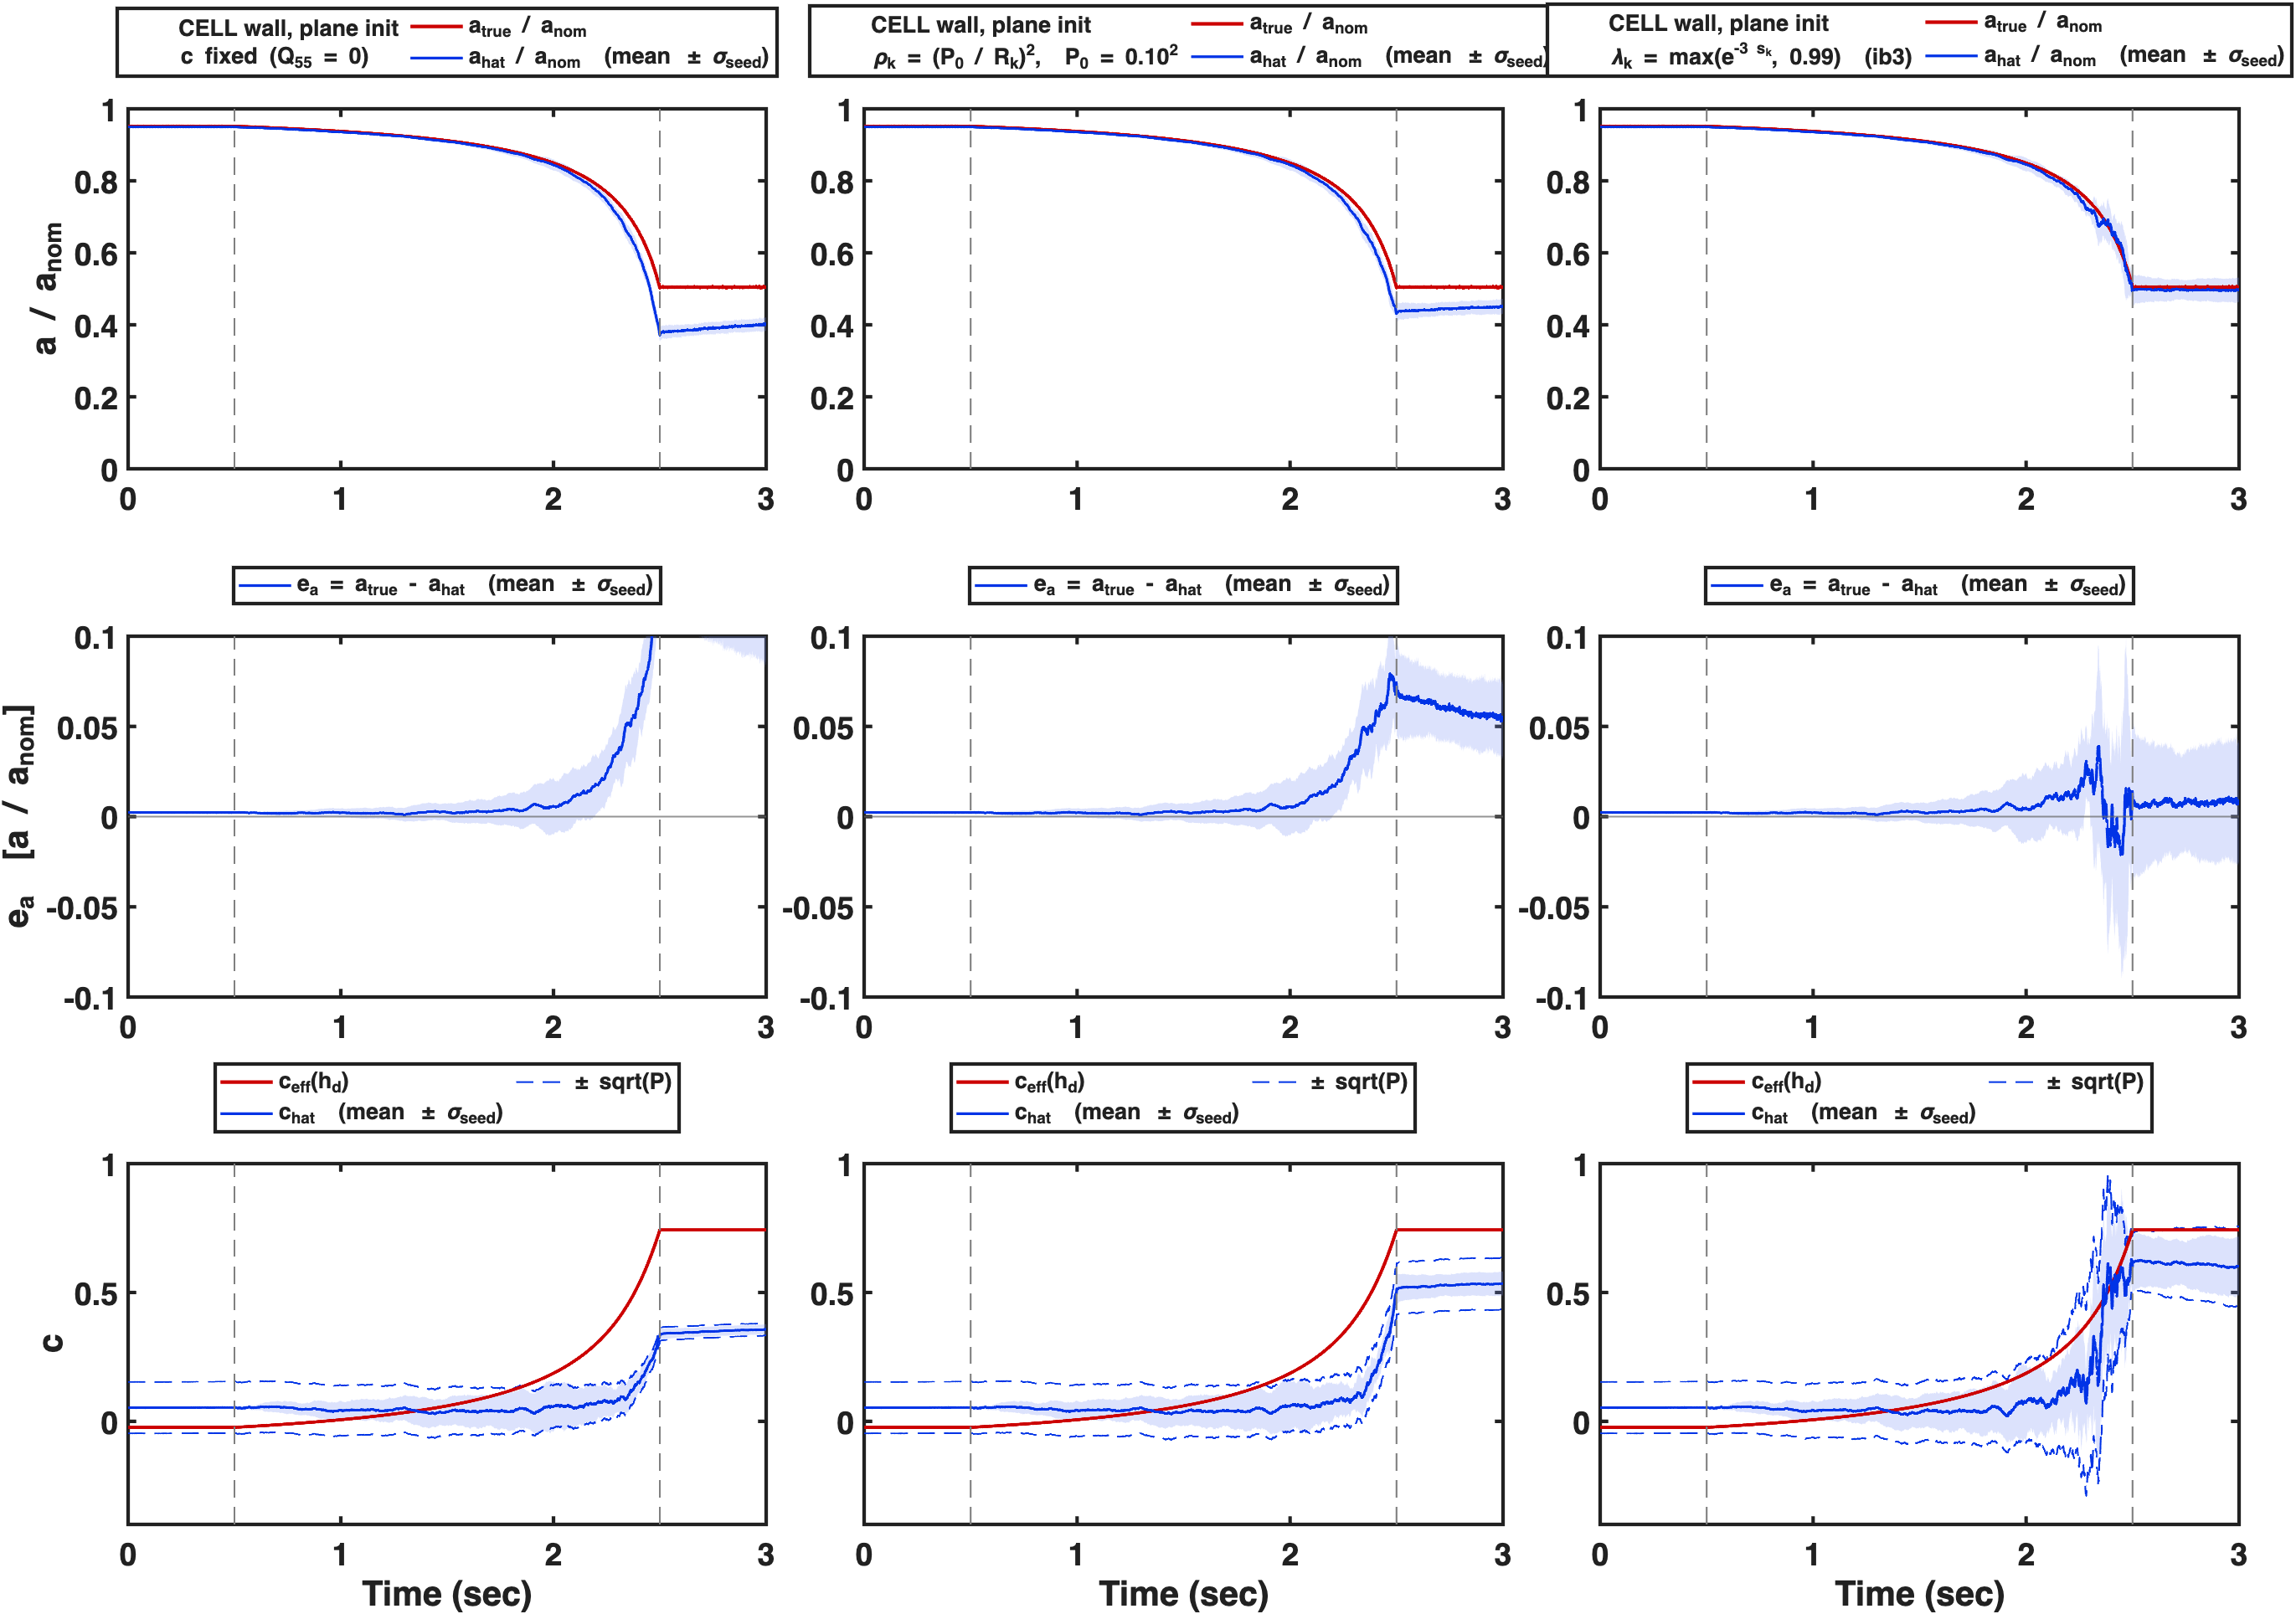
\includegraphics[width=\textwidth,height=0.86\textheight,keepaspectratio]{f1p2_cell_lf_compare_rho.png}\end{center}

\clearpage
%======================================================================
\section{Cell wall, plane init: the $P_0$ scan, $\sqrt{P_0} = 0.10 \mid 0.20 \mid 0.30$}
\begin{center}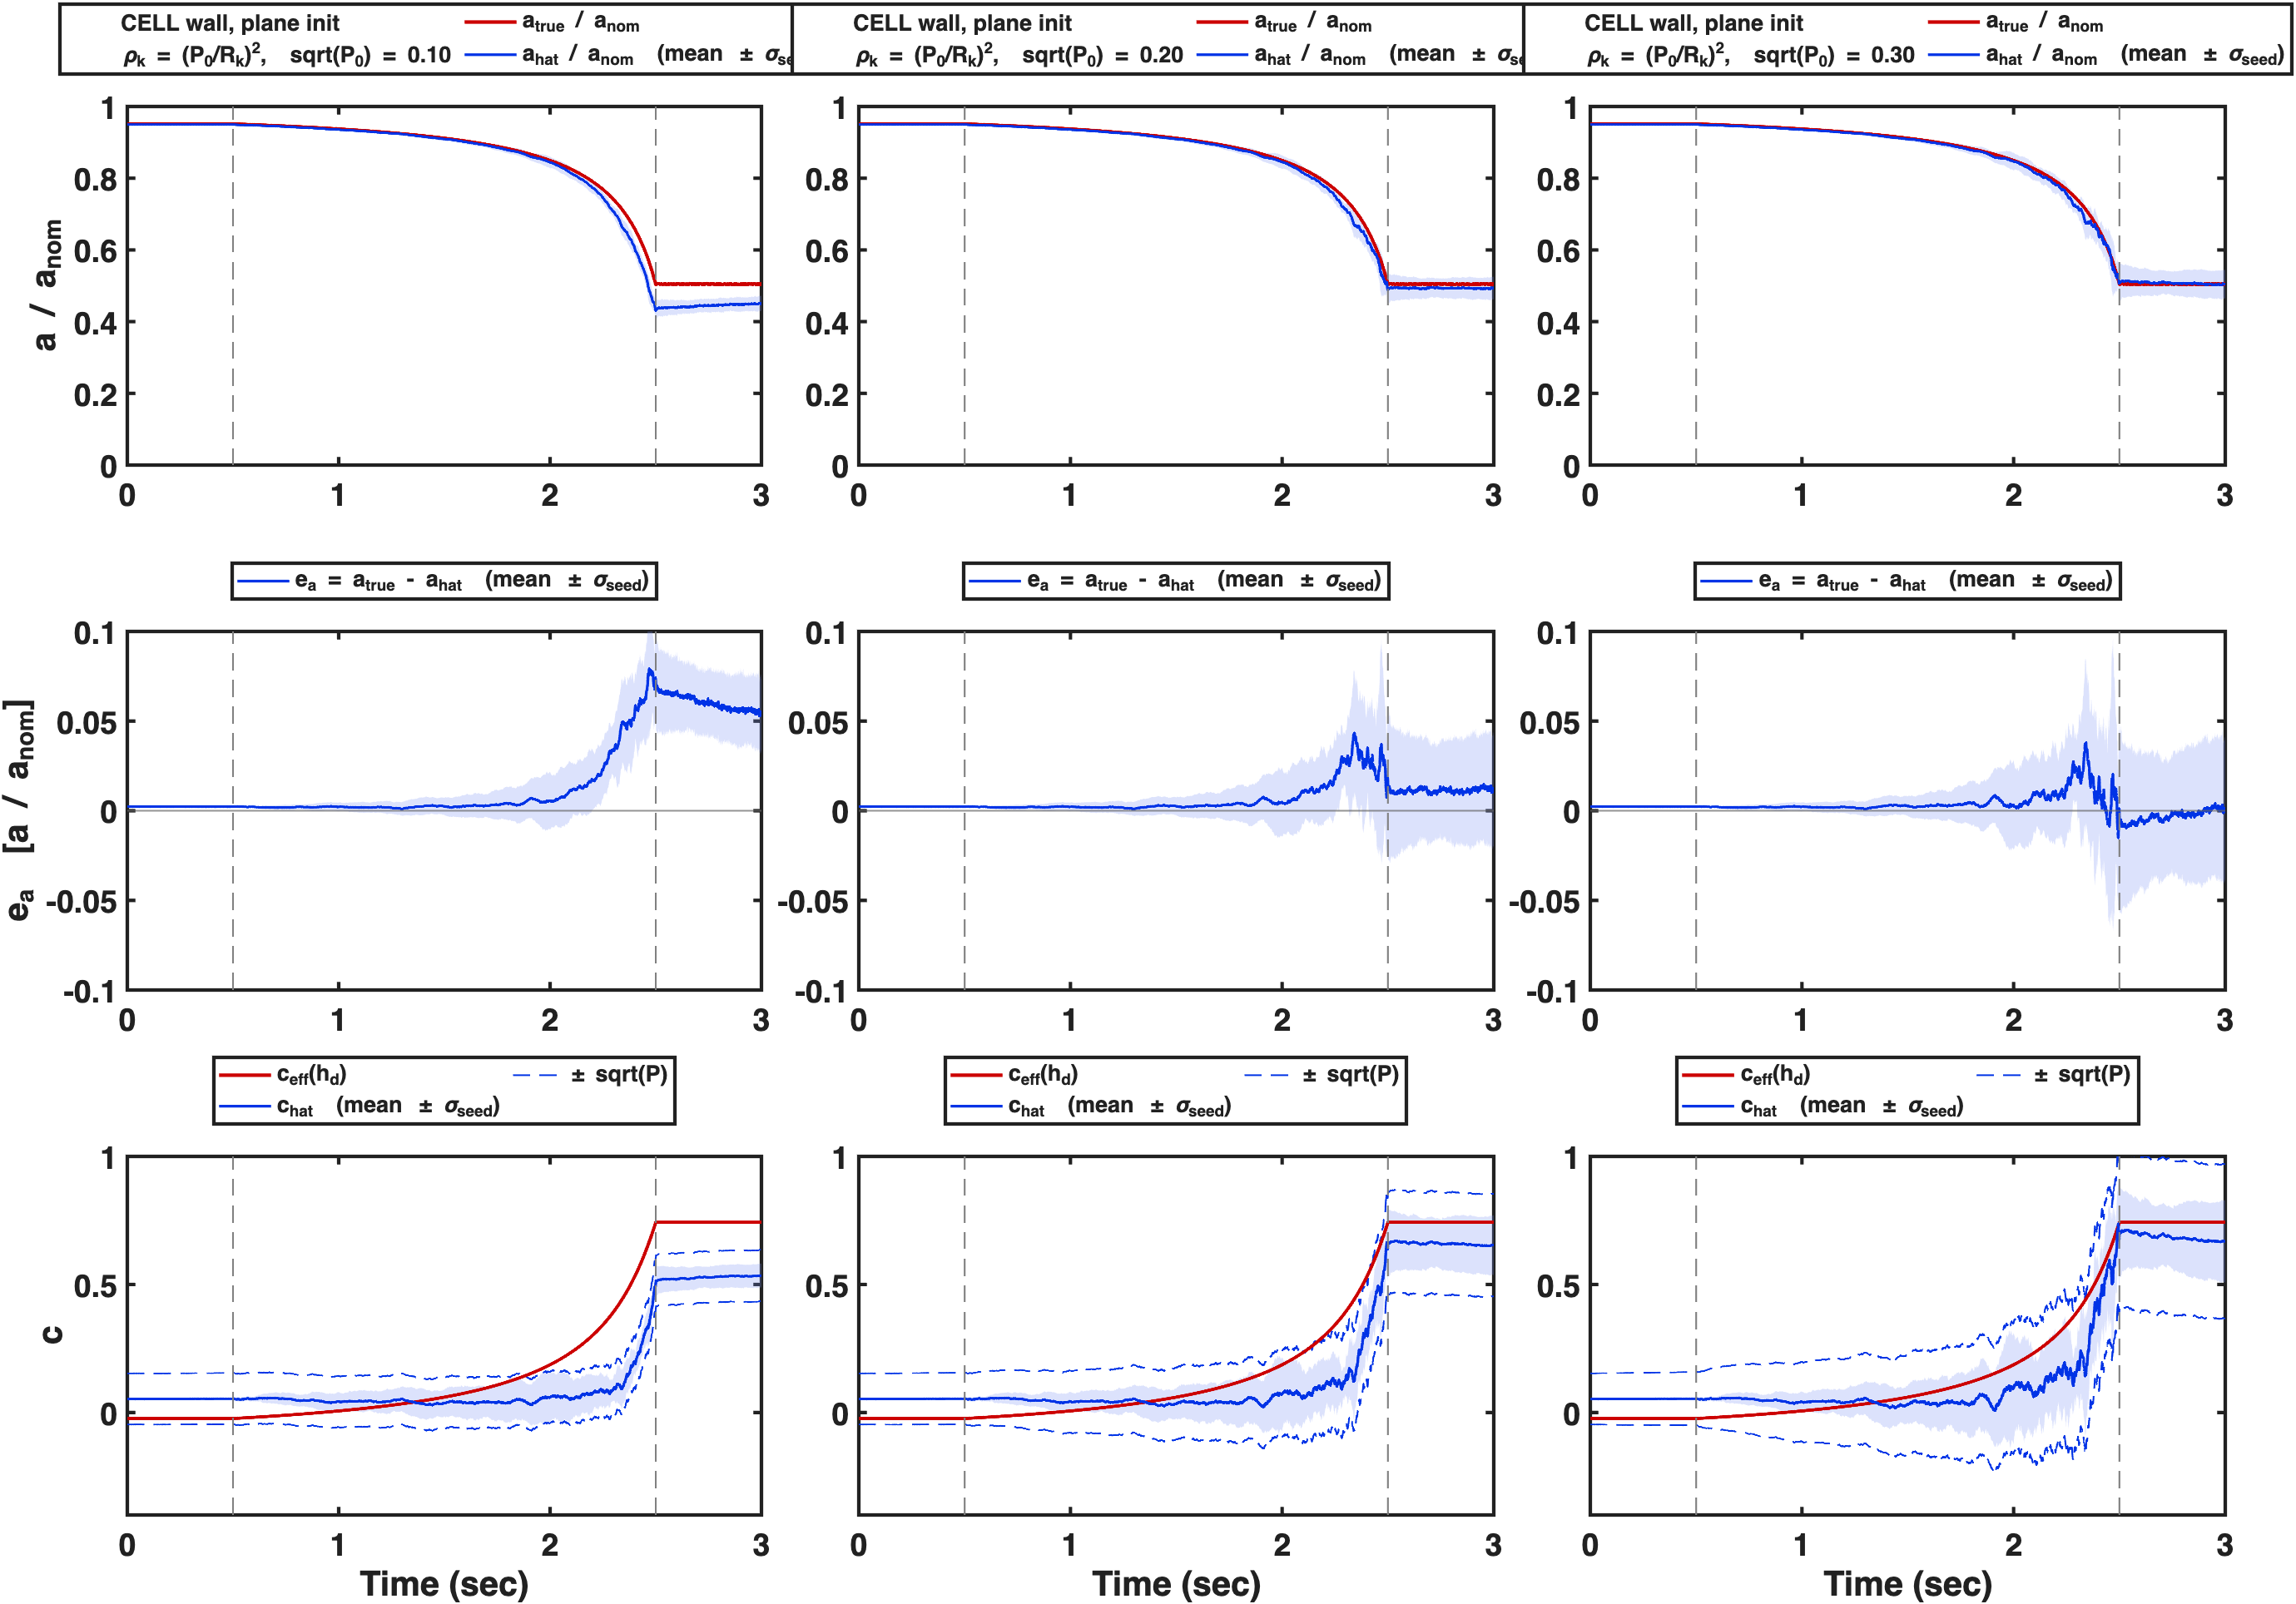
\includegraphics[width=\textwidth,height=0.86\textheight,keepaspectratio]{f1p2_cell_lf_compare_rhoscan.png}\end{center}

\clearpage
%======================================================================
\section{Cell wall, plane init, $\sqrt{P_0} = 0.20$: three descent speeds $T_d = 0.5 \mid 2 \mid 5$ s}
\begin{center}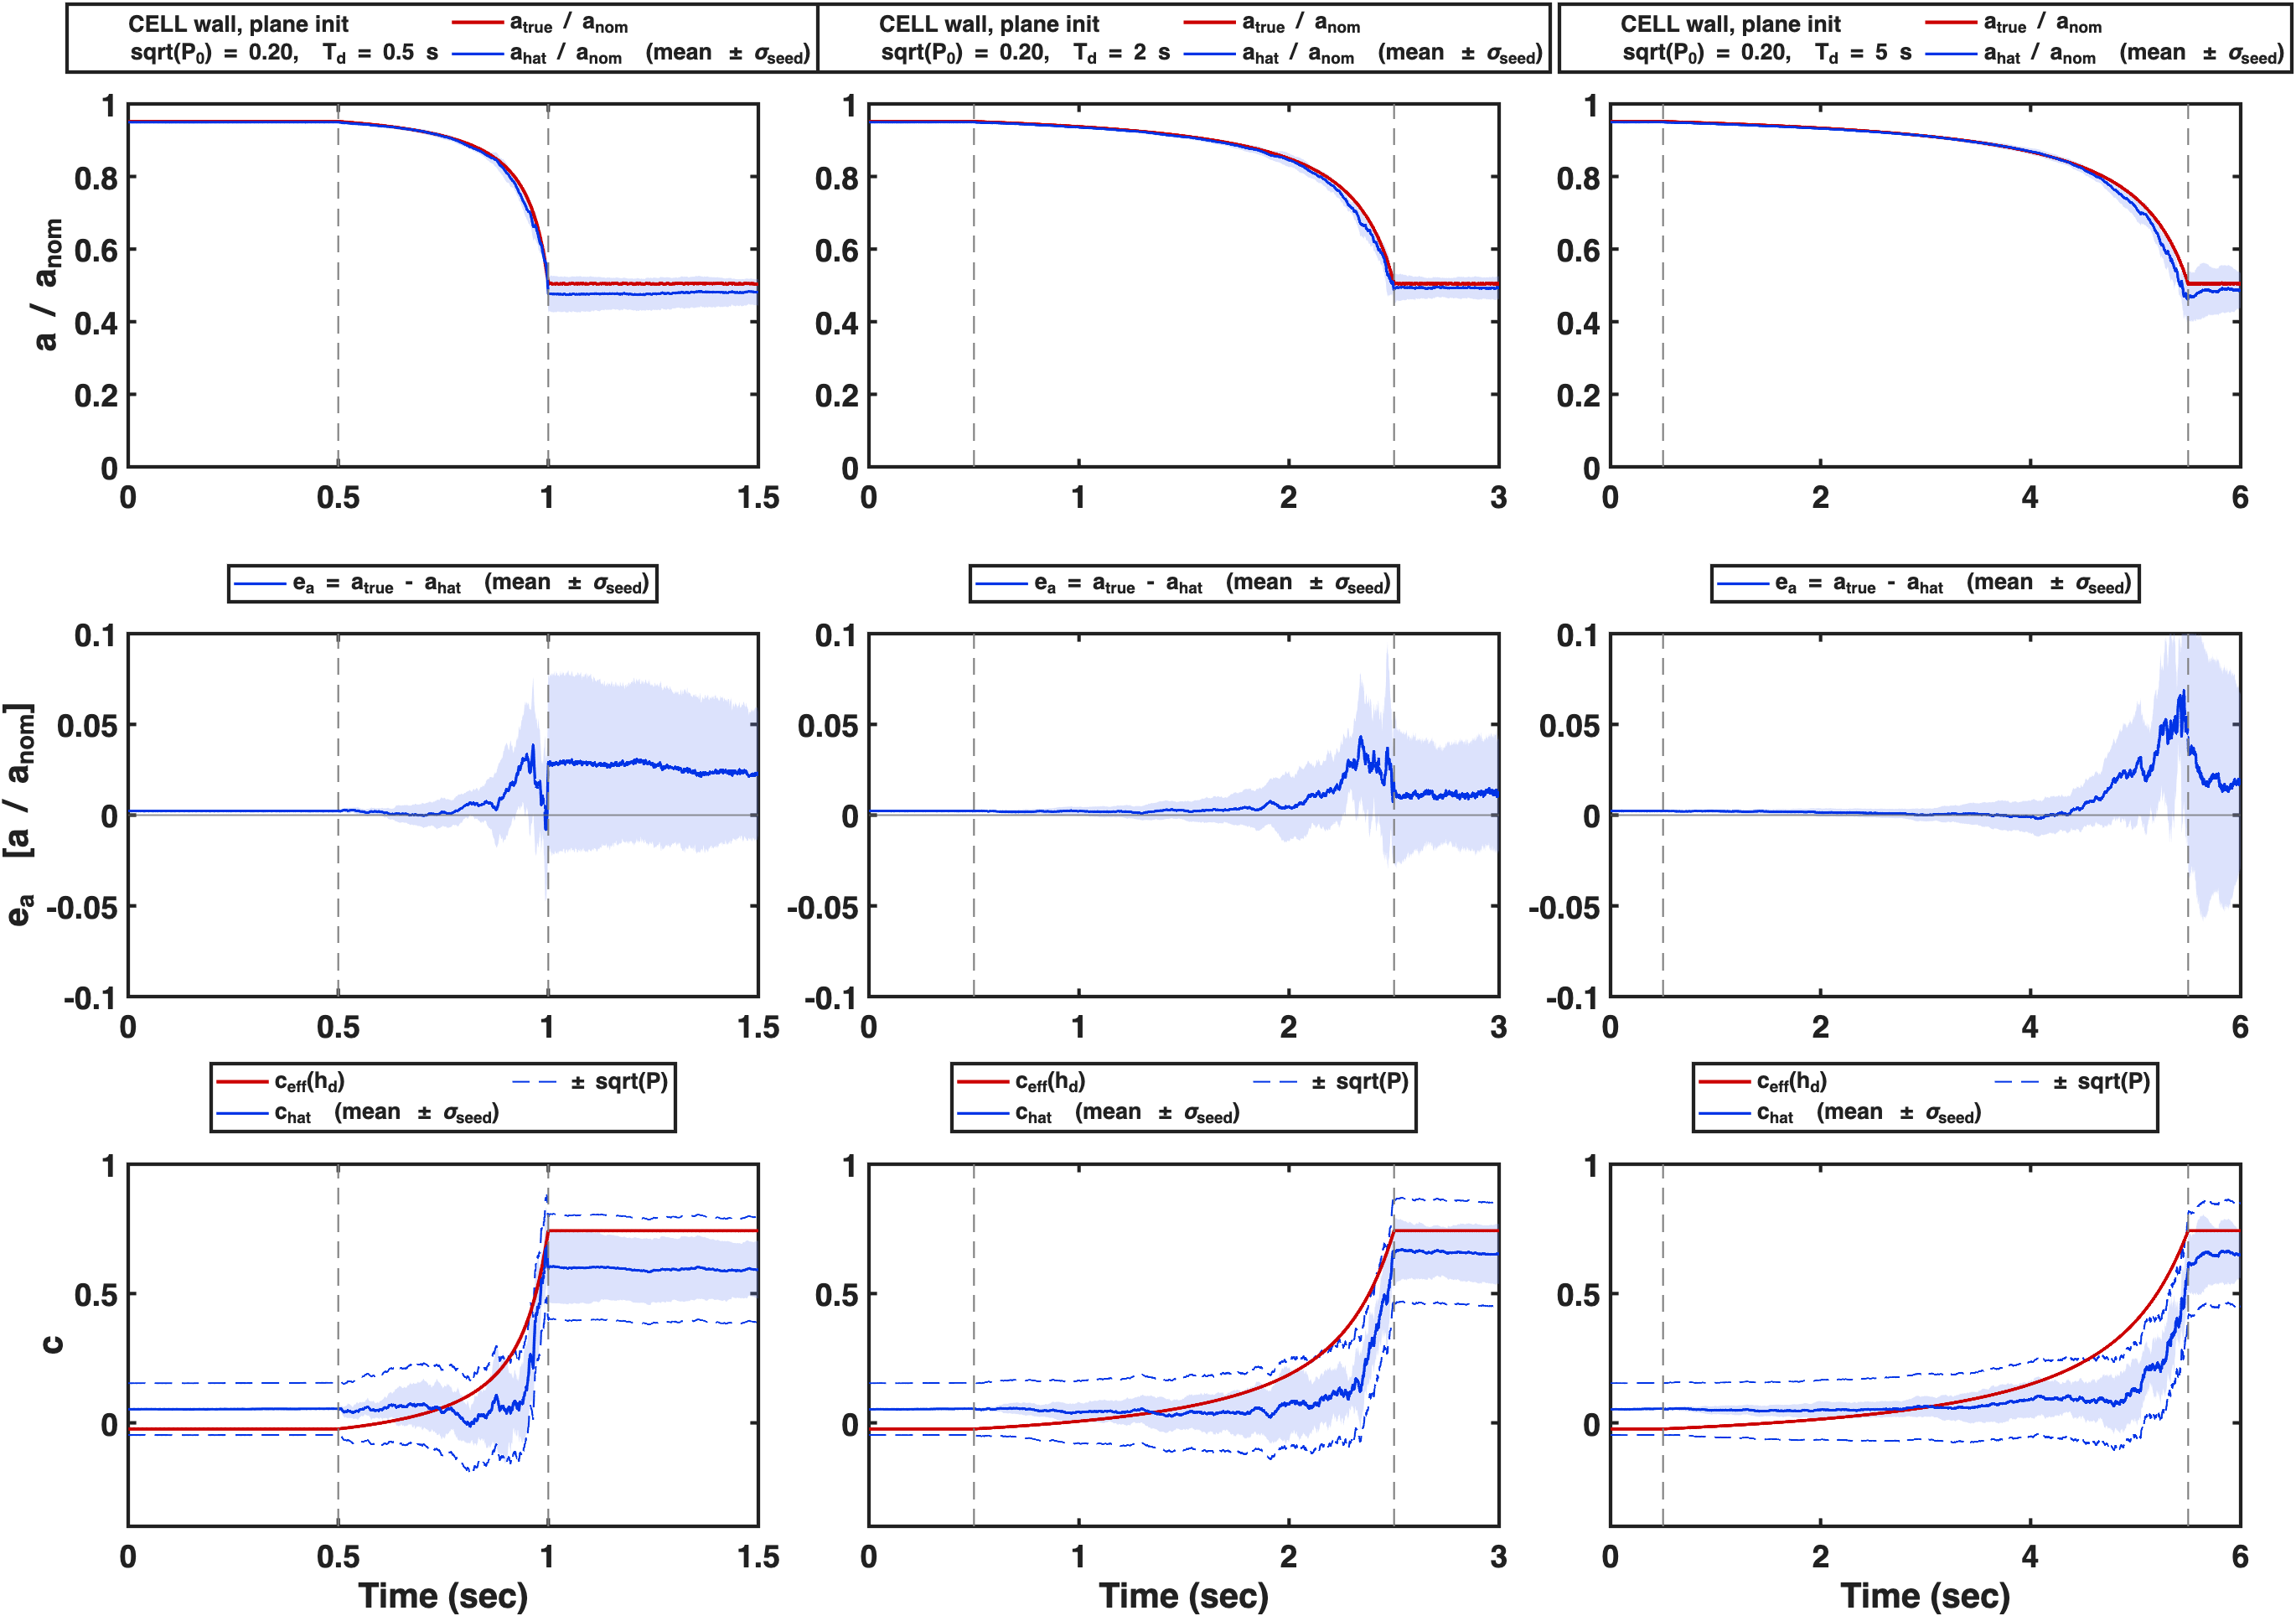
\includegraphics[width=\textwidth,height=0.86\textheight,keepaspectratio]{f1p2_cell_lf_compare_rho20_speed.png}\end{center}

\clearpage
%======================================================================
\section{Cell wall, plane init, $Q_{55} = 0$ (base): the same three speeds}
\begin{center}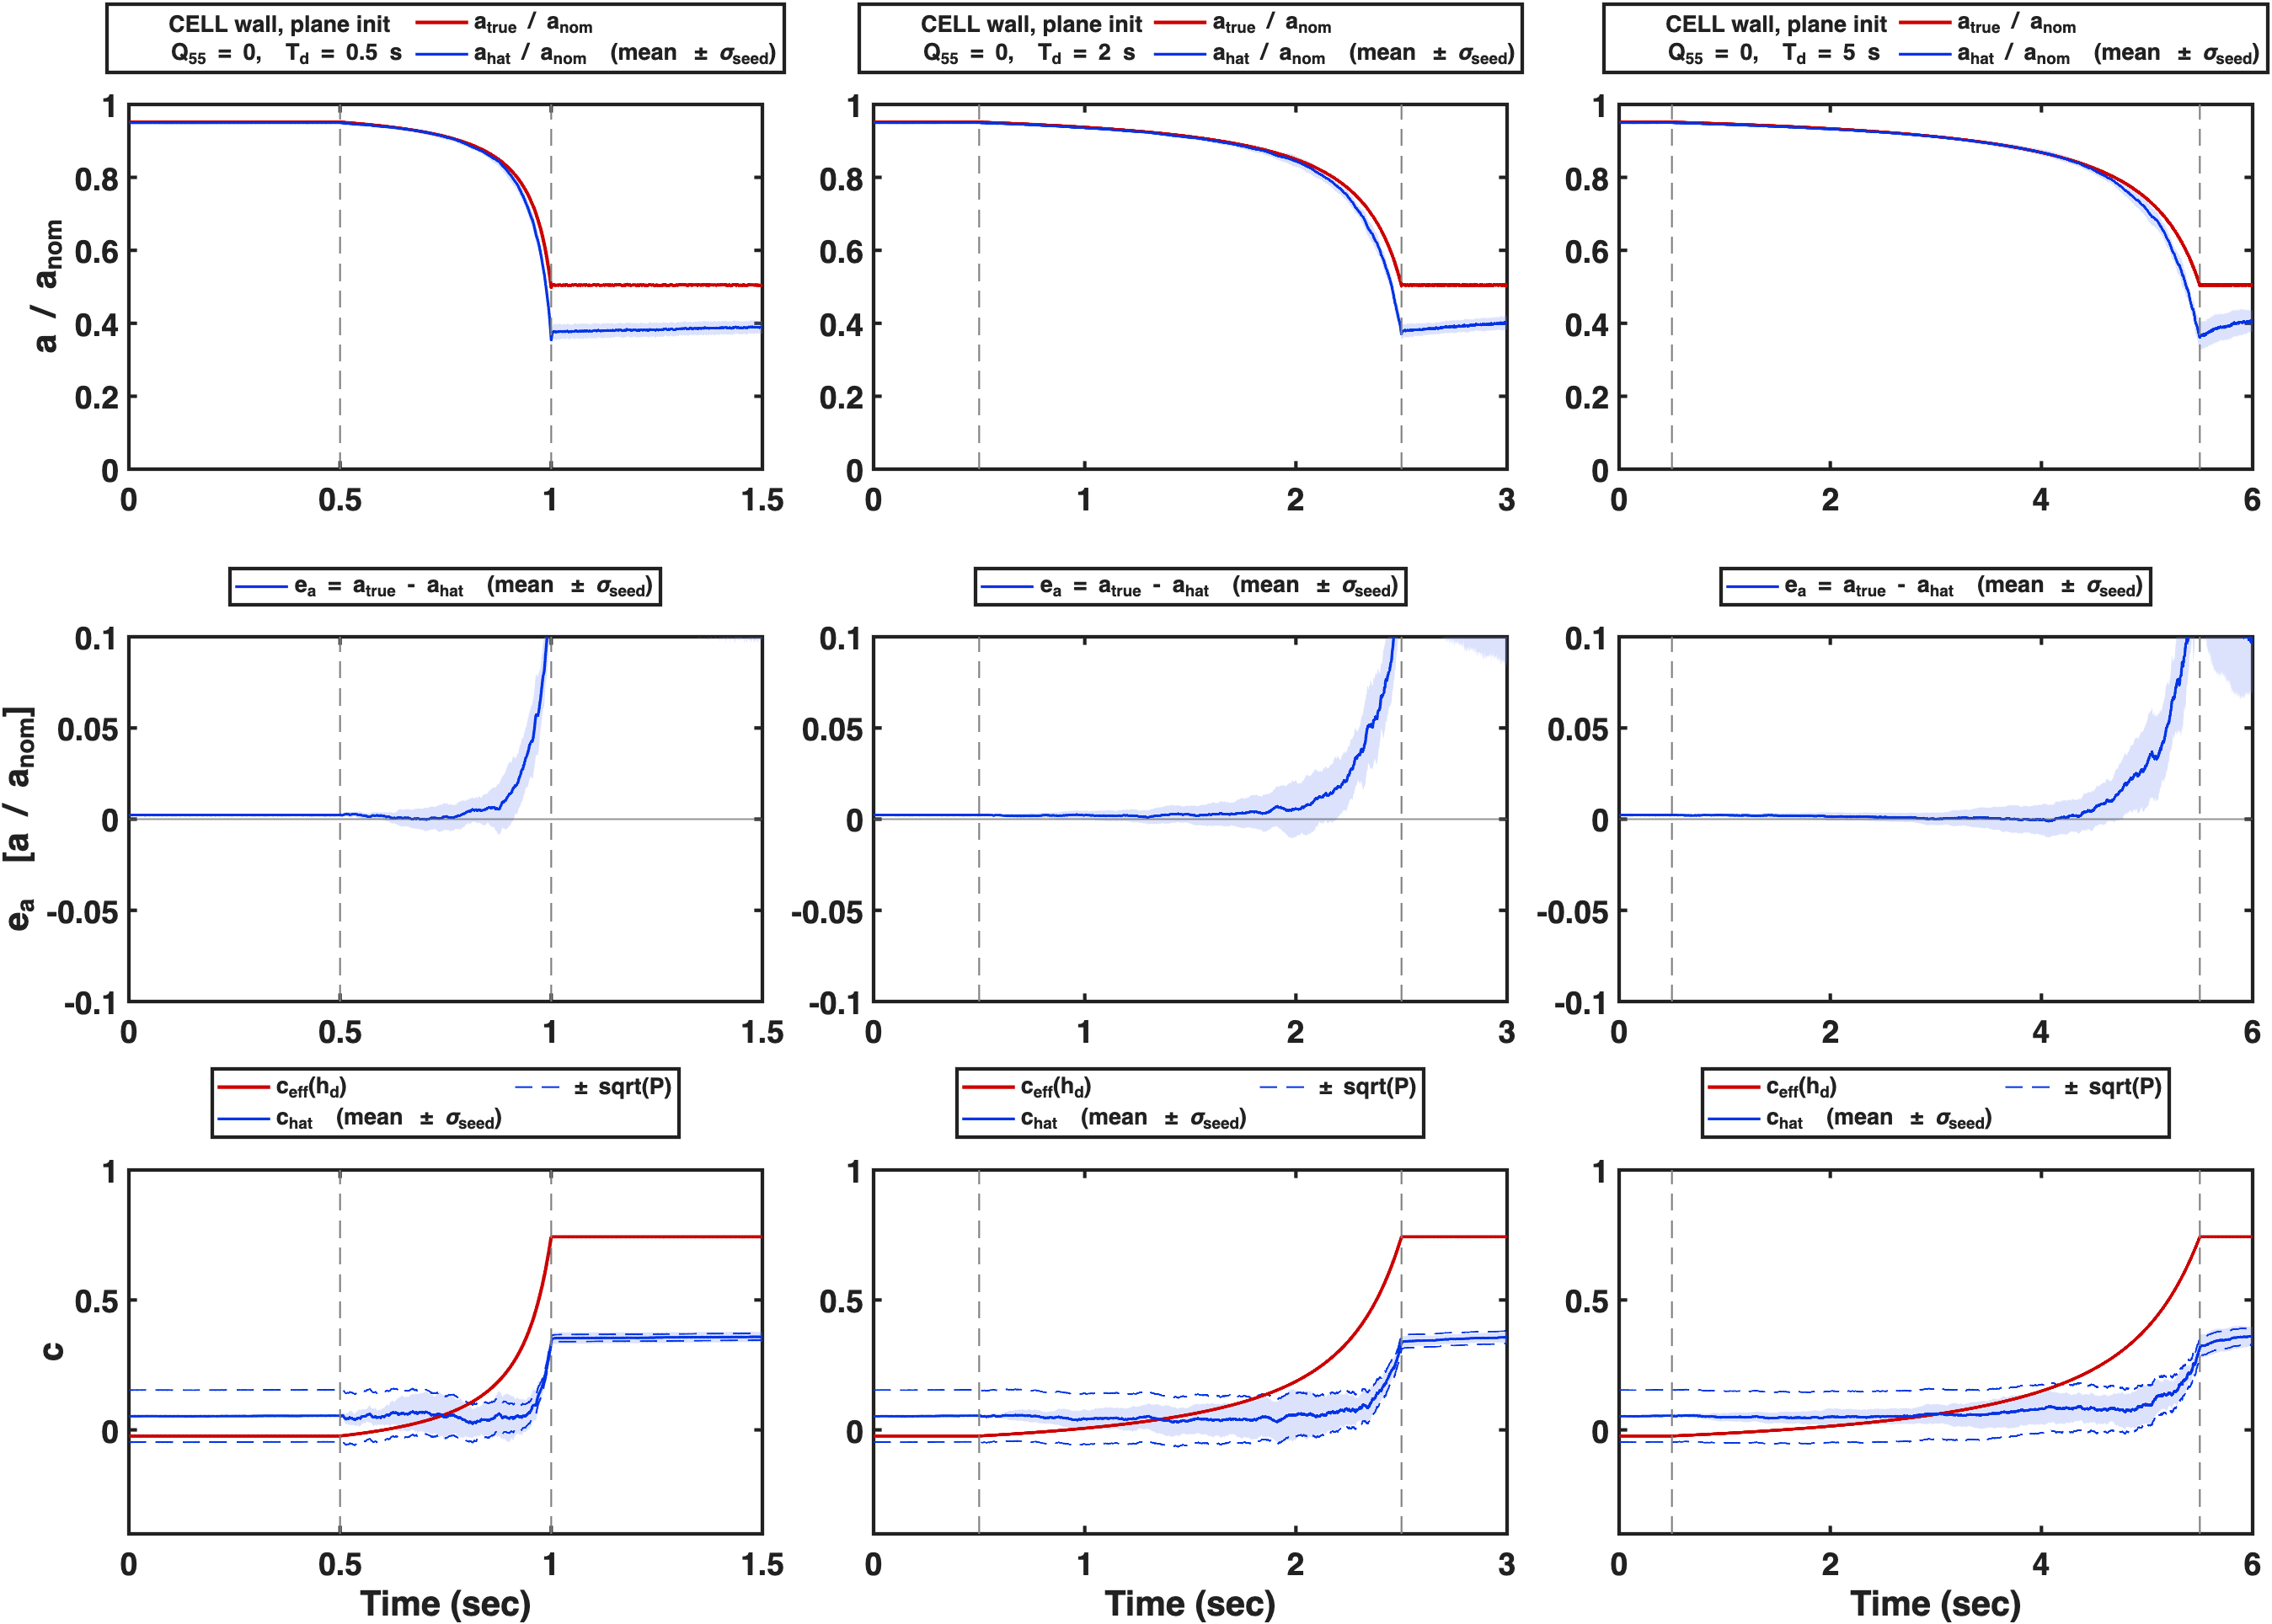
\includegraphics[width=\textwidth,height=0.86\textheight,keepaspectratio]{f1p2_cell_lf_compare_base_speed.png}\end{center}

\clearpage
%======================================================================
\section{Plane | cell, ratio $\sqrt{P_0} = 0.20$: $I_k$, $Q_{55}$, $\rho_k$, $N_k$, $\sqrt{P_{55}}$ along the run}
\begin{center}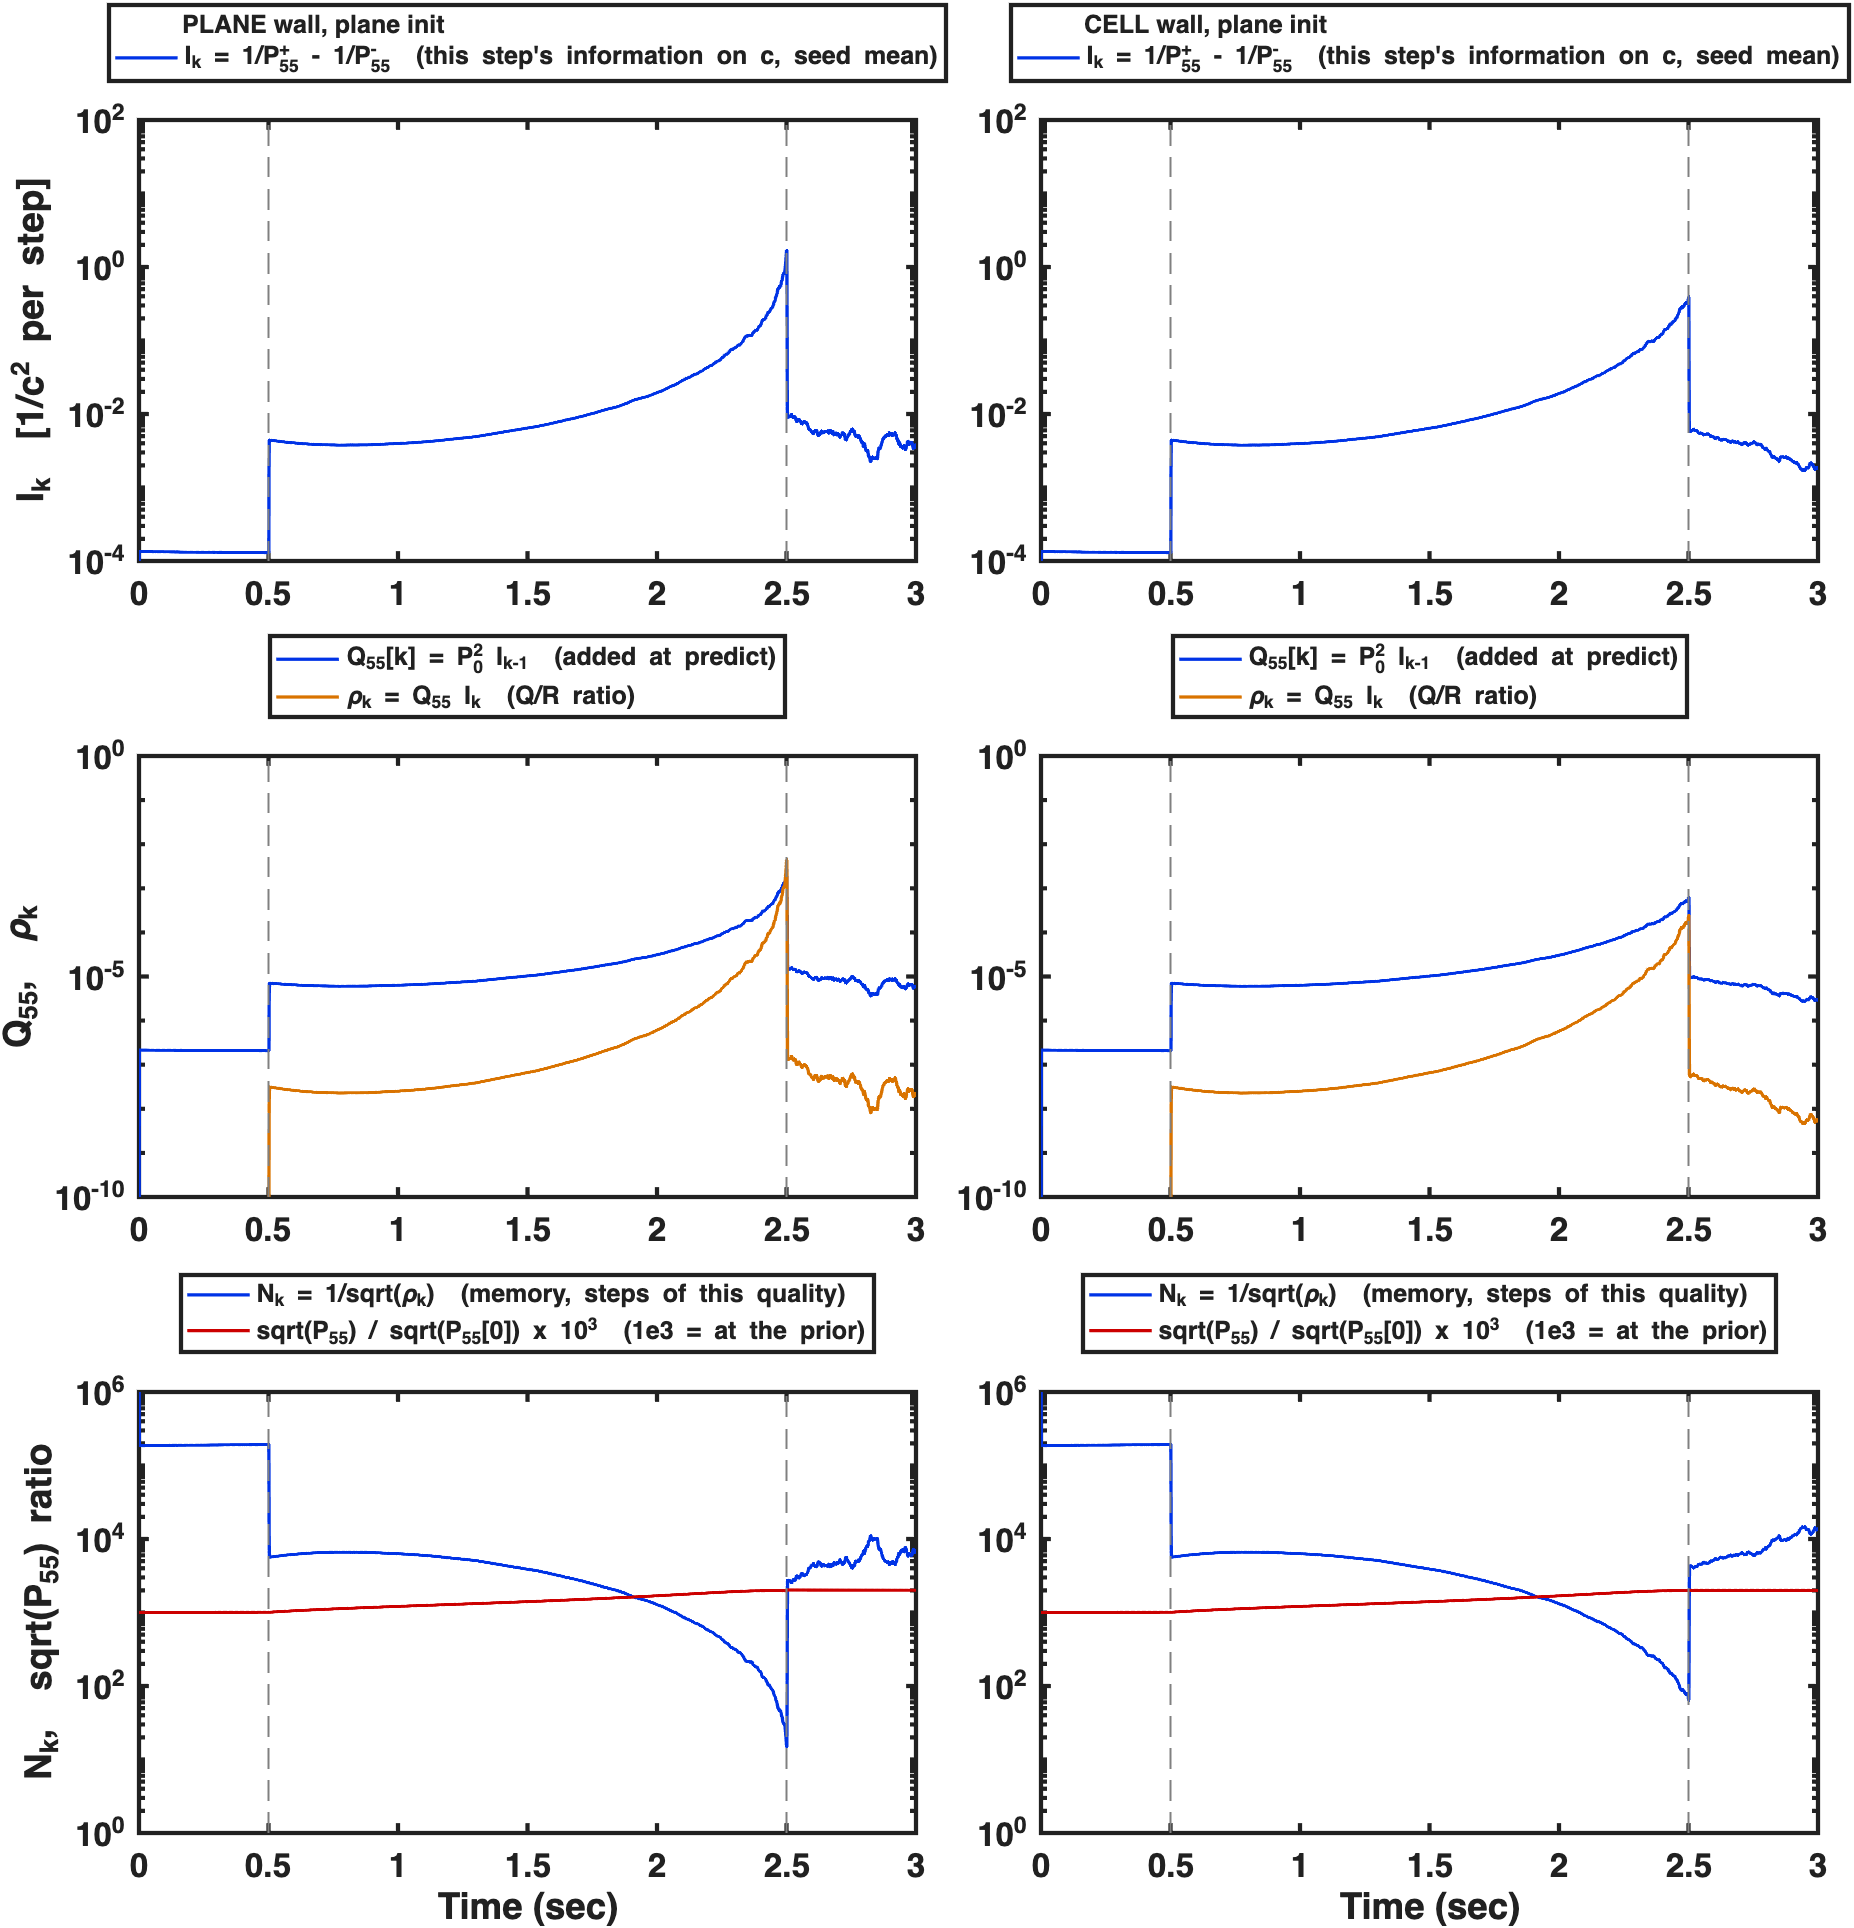
\includegraphics[width=\textwidth,height=0.86\textheight,keepaspectratio]{rho_diag_walls_sig010_rho20_ramp2.png}\end{center}

\clearpage
%======================================================================
\section{The opponents (cell, ramp 2 s): ratio $\sqrt{P_0} = 0.2$ | constant $\rho = 1/25^2$ | constant $\rho = 1/100^2$}
\[
Q_{55} = \frac{\rho}{I_k}, \qquad P_{55}^{\mathrm{eq}} = \frac{\sqrt{\rho}}{I_k} \;\to\; \infty \ (I_k \to 0)
\]
\begin{center}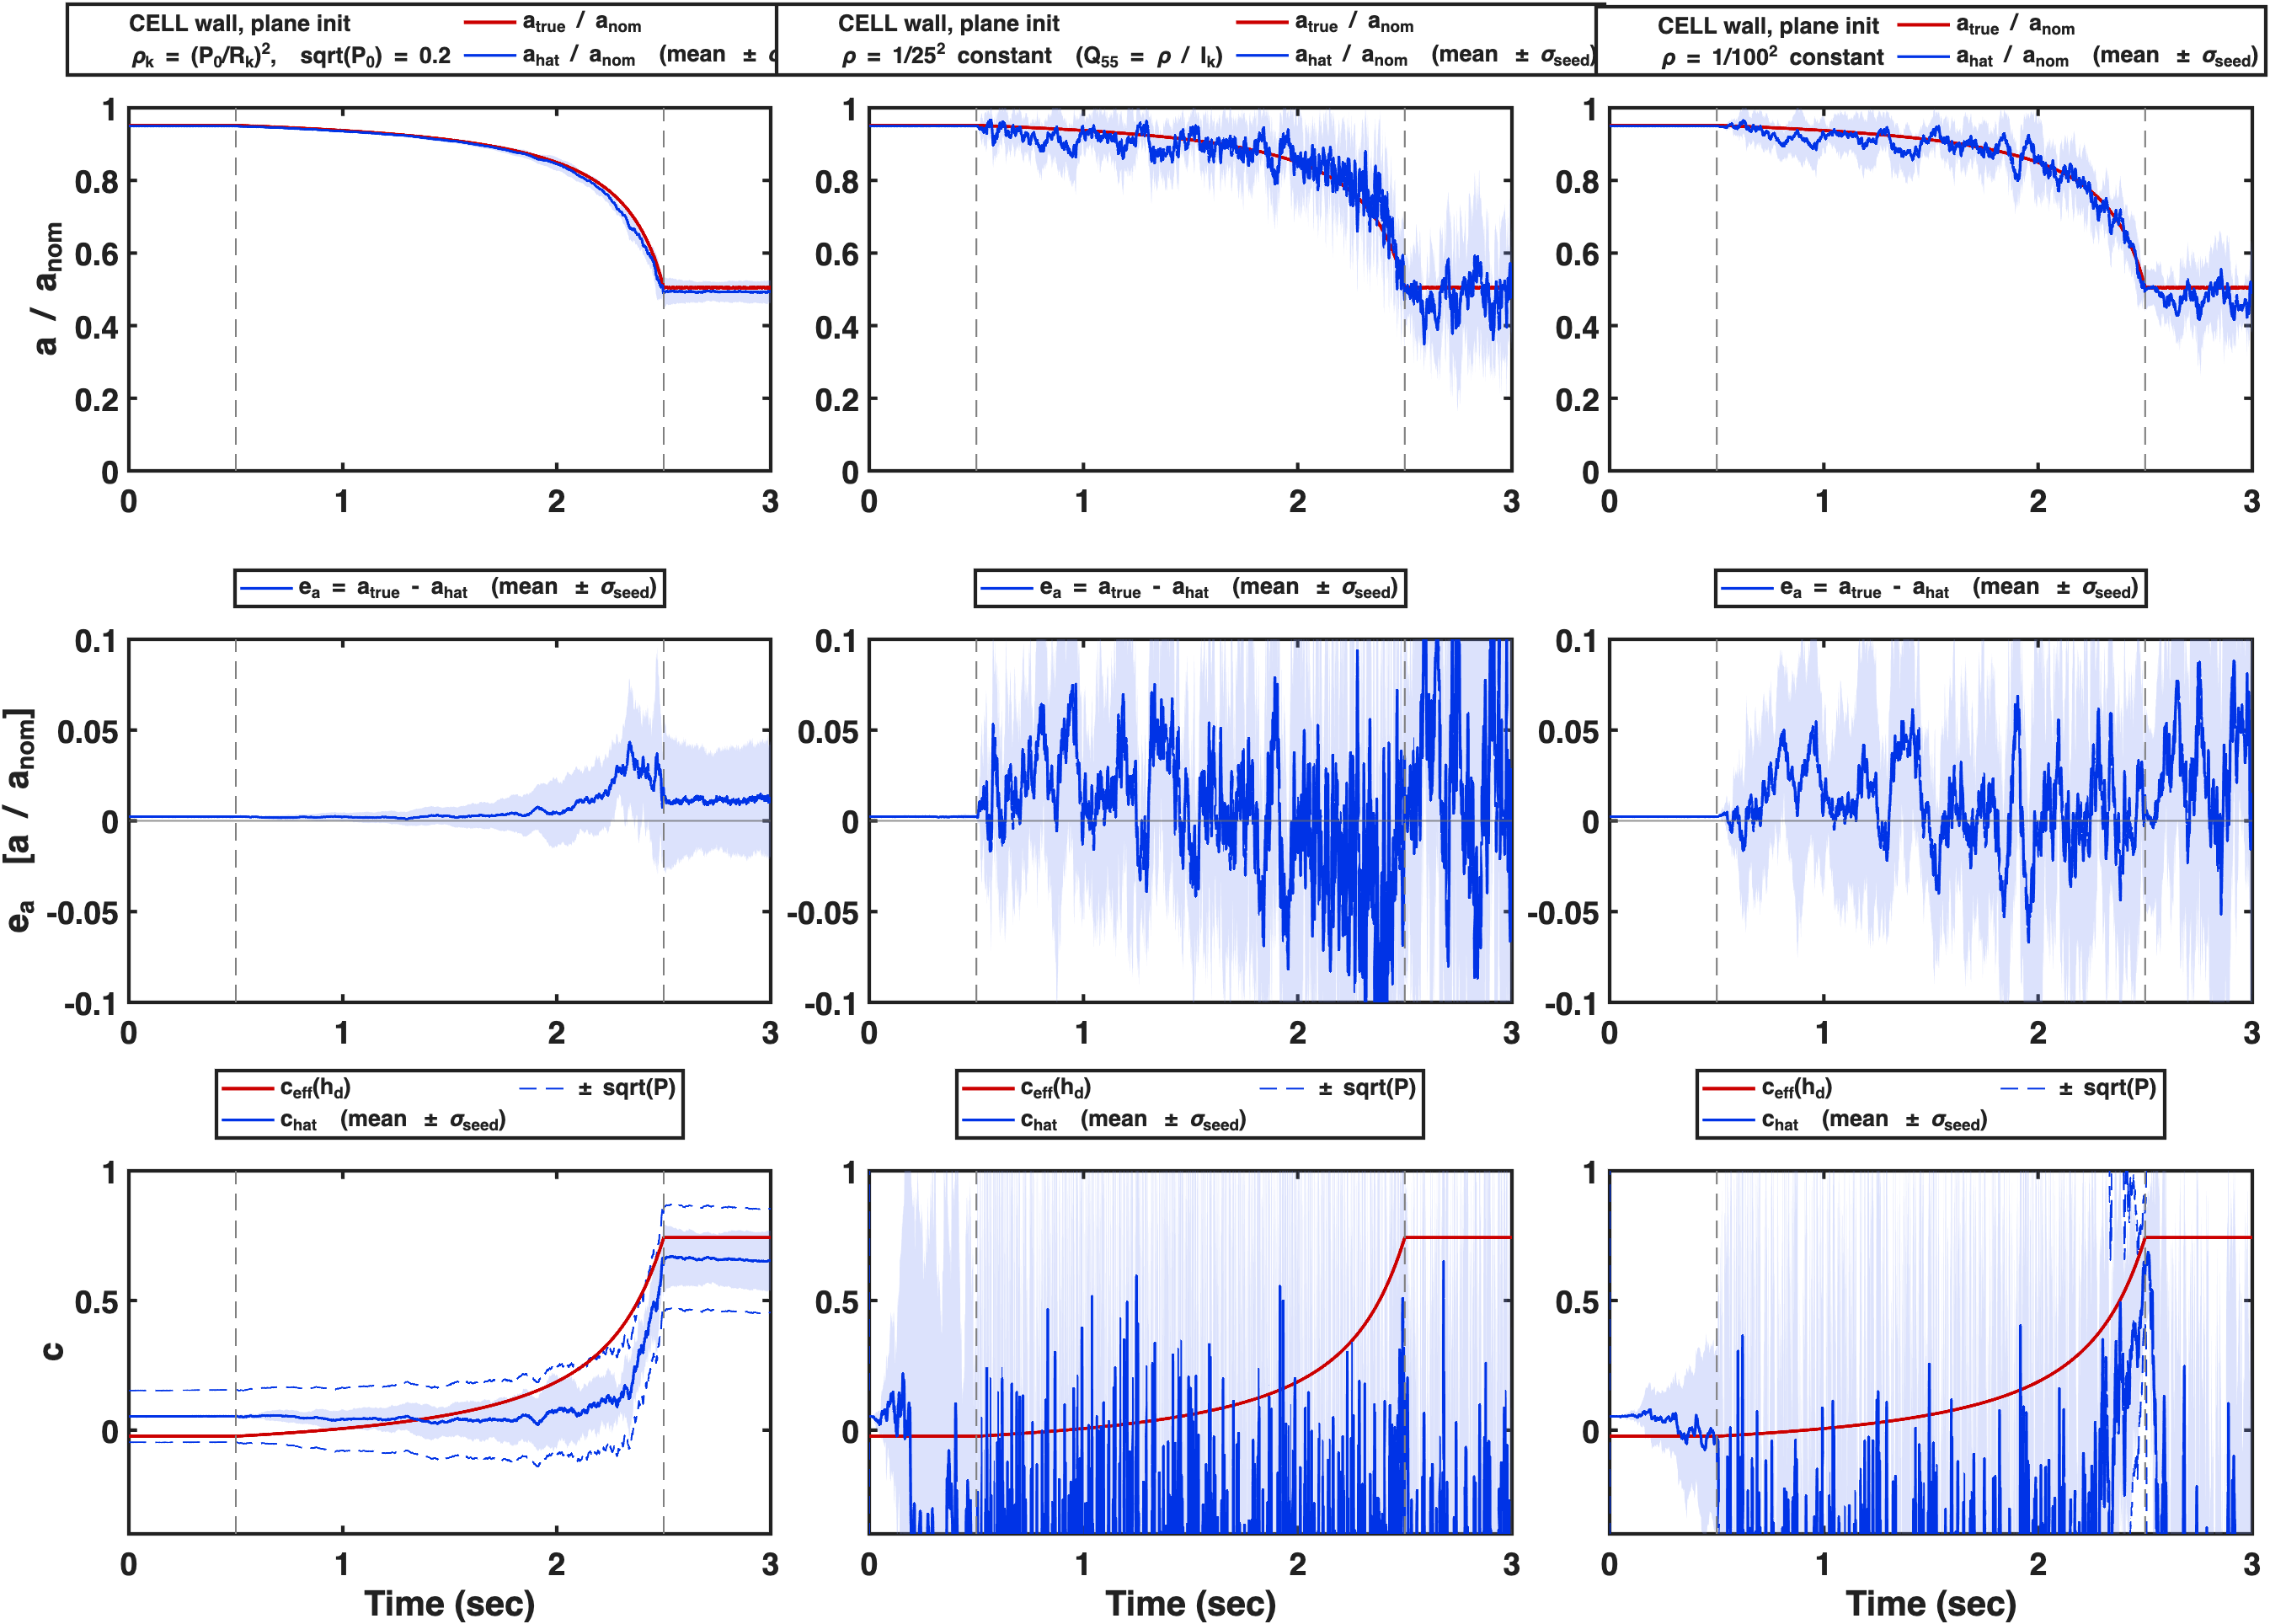
\includegraphics[width=\textwidth,height=0.80\textheight,keepaspectratio]{f1p2_cell_lf_compare_rhoconst.png}\end{center}

\clearpage
%======================================================================
\section{The opponents (cell, ramp 2 s): ratio | $Q_{55} = 0.03\,R_2$ | $Q_{55} = 0.3\,R_2$}
\[
Q_{55} = \rho\,R_2[k], \qquad P_{55}^{\mathrm{eq}} = \sqrt{\frac{\rho R_2[k]}{I_k}} \qquad (R_2 \text{ large where } I_k \text{ small: far field, hold})
\]
\begin{center}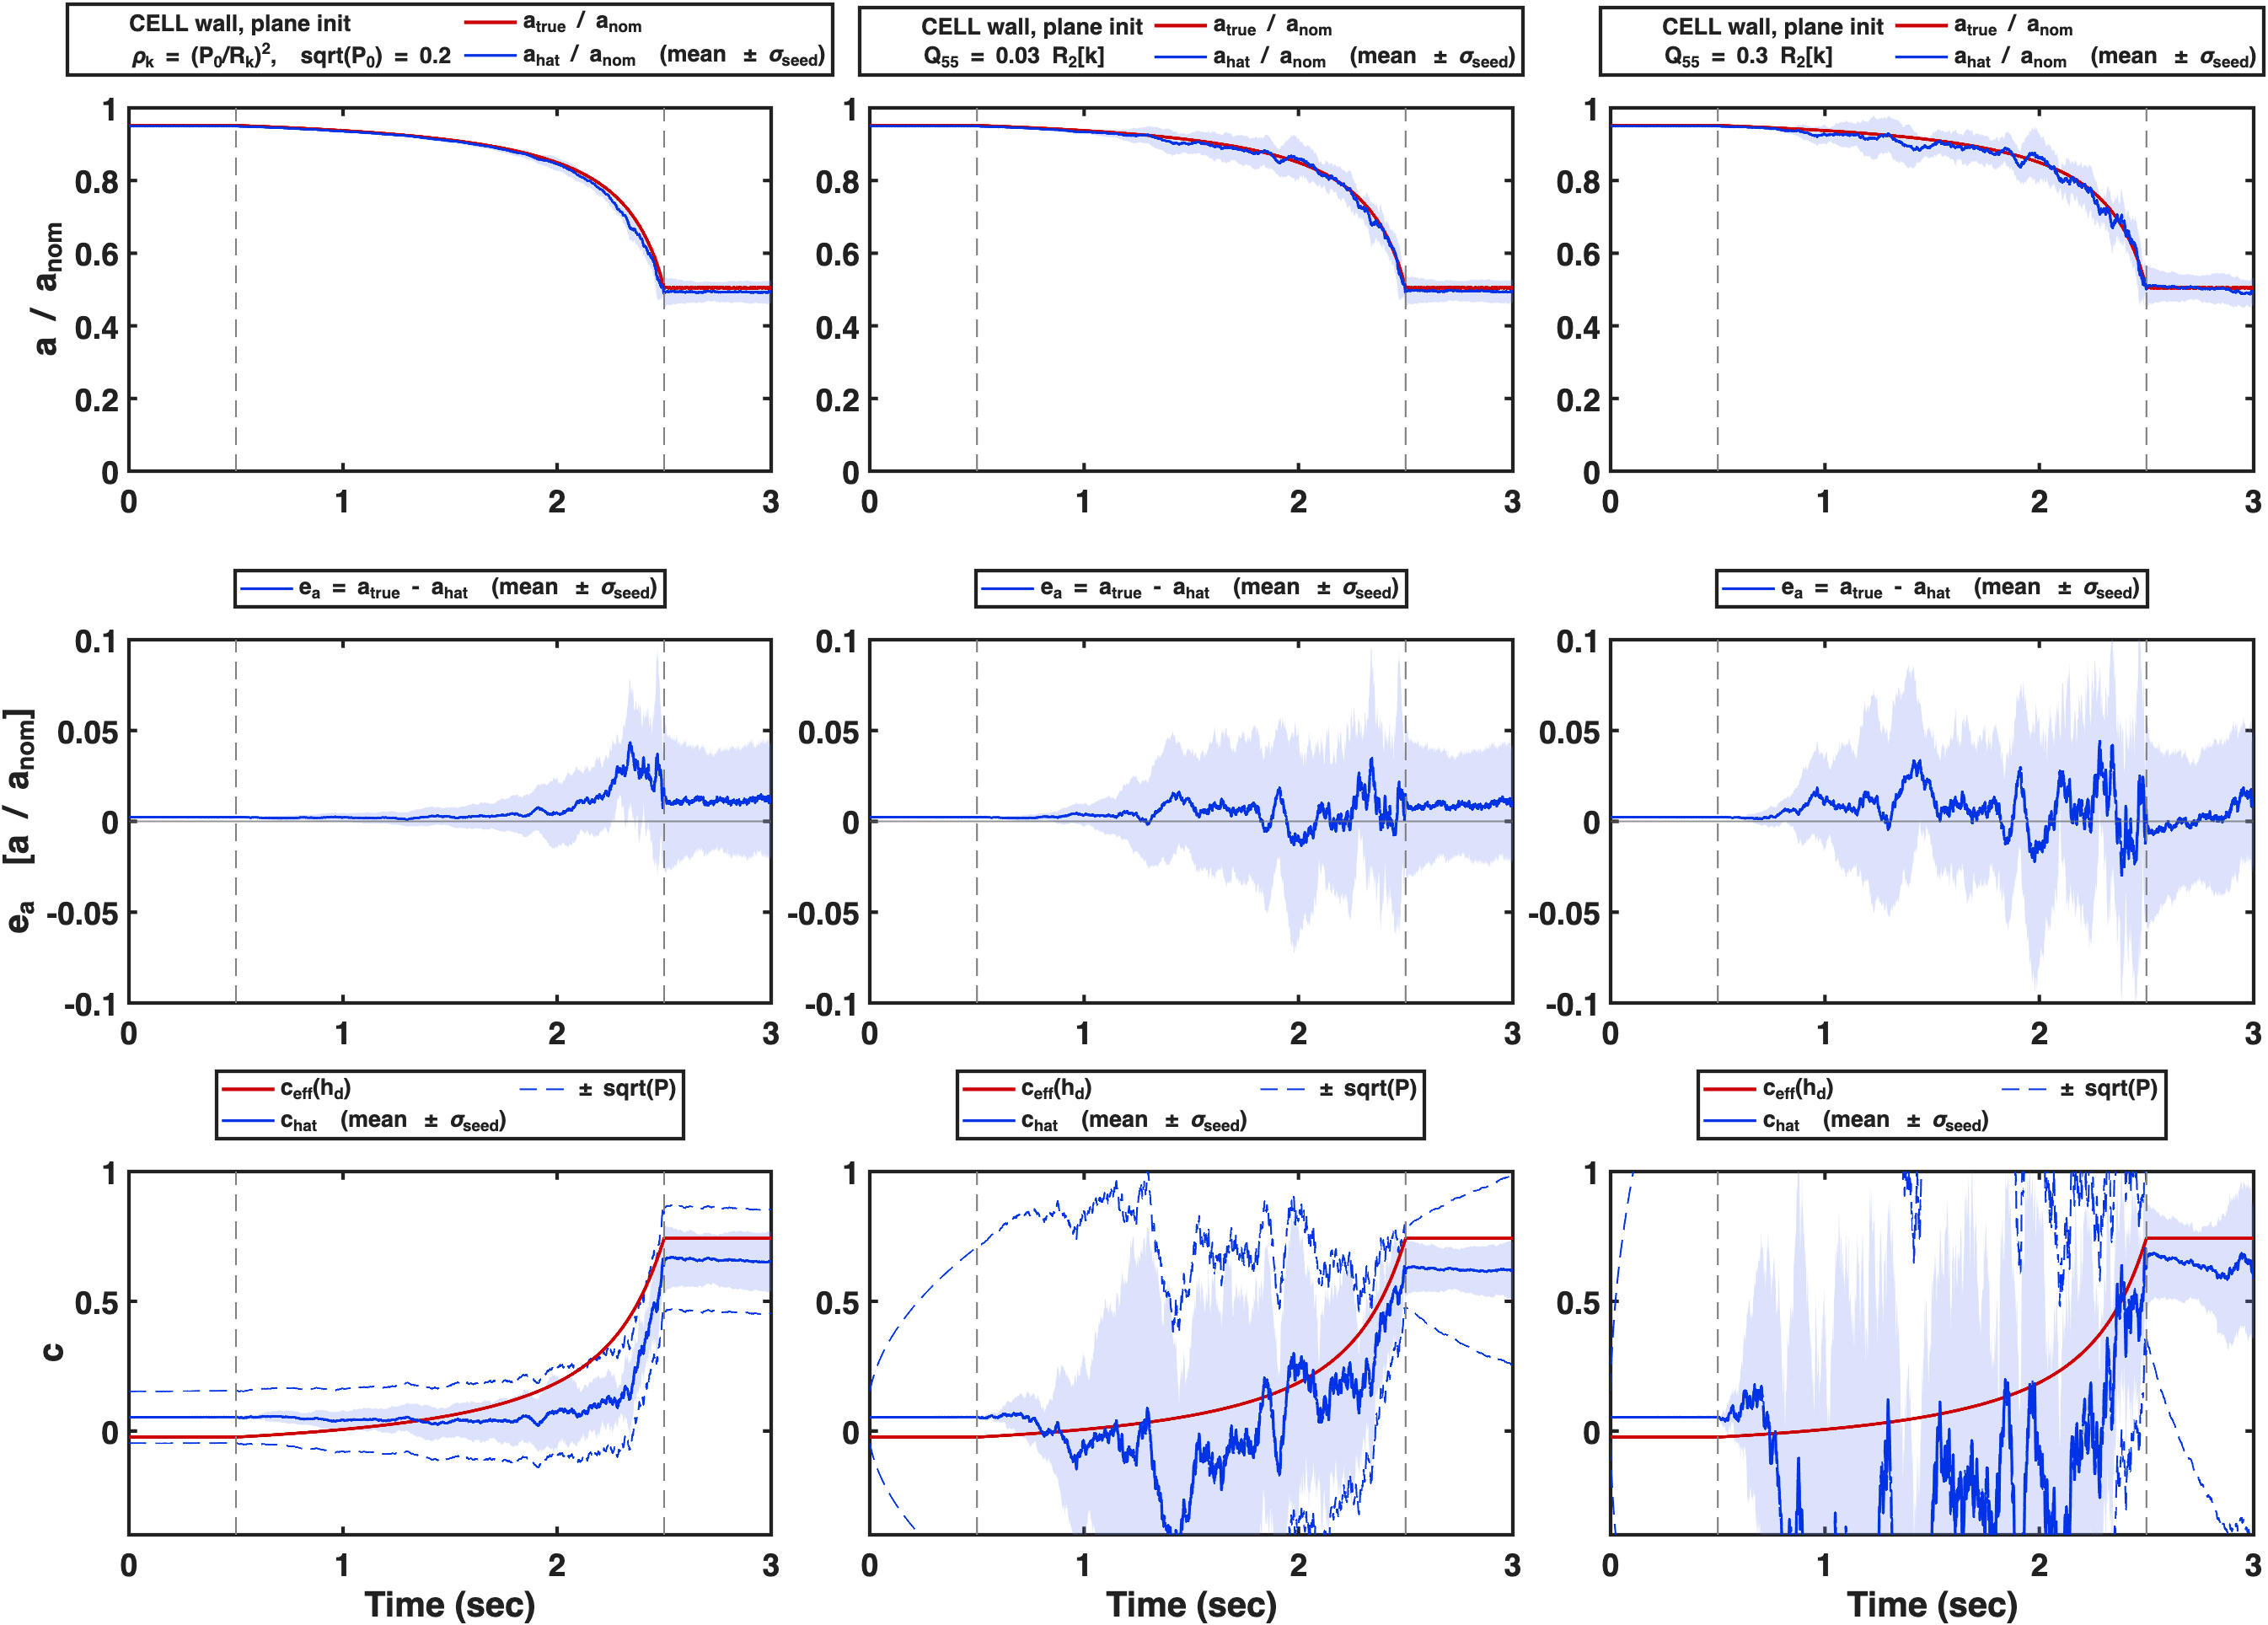
\includegraphics[width=\textwidth,height=0.80\textheight,keepaspectratio]{f1p2_cell_lf_compare_r2ratio.png}\end{center}

\clearpage
%======================================================================
\section{What $\hat c$ is compared with on the oscillation: the open-loop potential of a constant $c$}
\[
e_{\ba}(h) = \int_{h_{\mathrm{top}}}^{h} \big(c_{\mathrm{eff}}(h') - \ch\big)\,\frac{dh'}{h'^{2}}, \qquad
c^{*}_{\mathrm{band}} = \frac{\int_{\mathrm{band}} c_{\mathrm{eff}}\,dh/h^{2}}{\int_{\mathrm{band}} dh/h^{2}}
\]
\[
1.10\text{--}3.32\,R:\ c^{*}_{\mathrm{band}} = 0.60,\ \text{in-band extreme } 0.026; \qquad 1.05\text{--}2.0\,R:\ 0.67,\ 0.011
\]
\begin{center}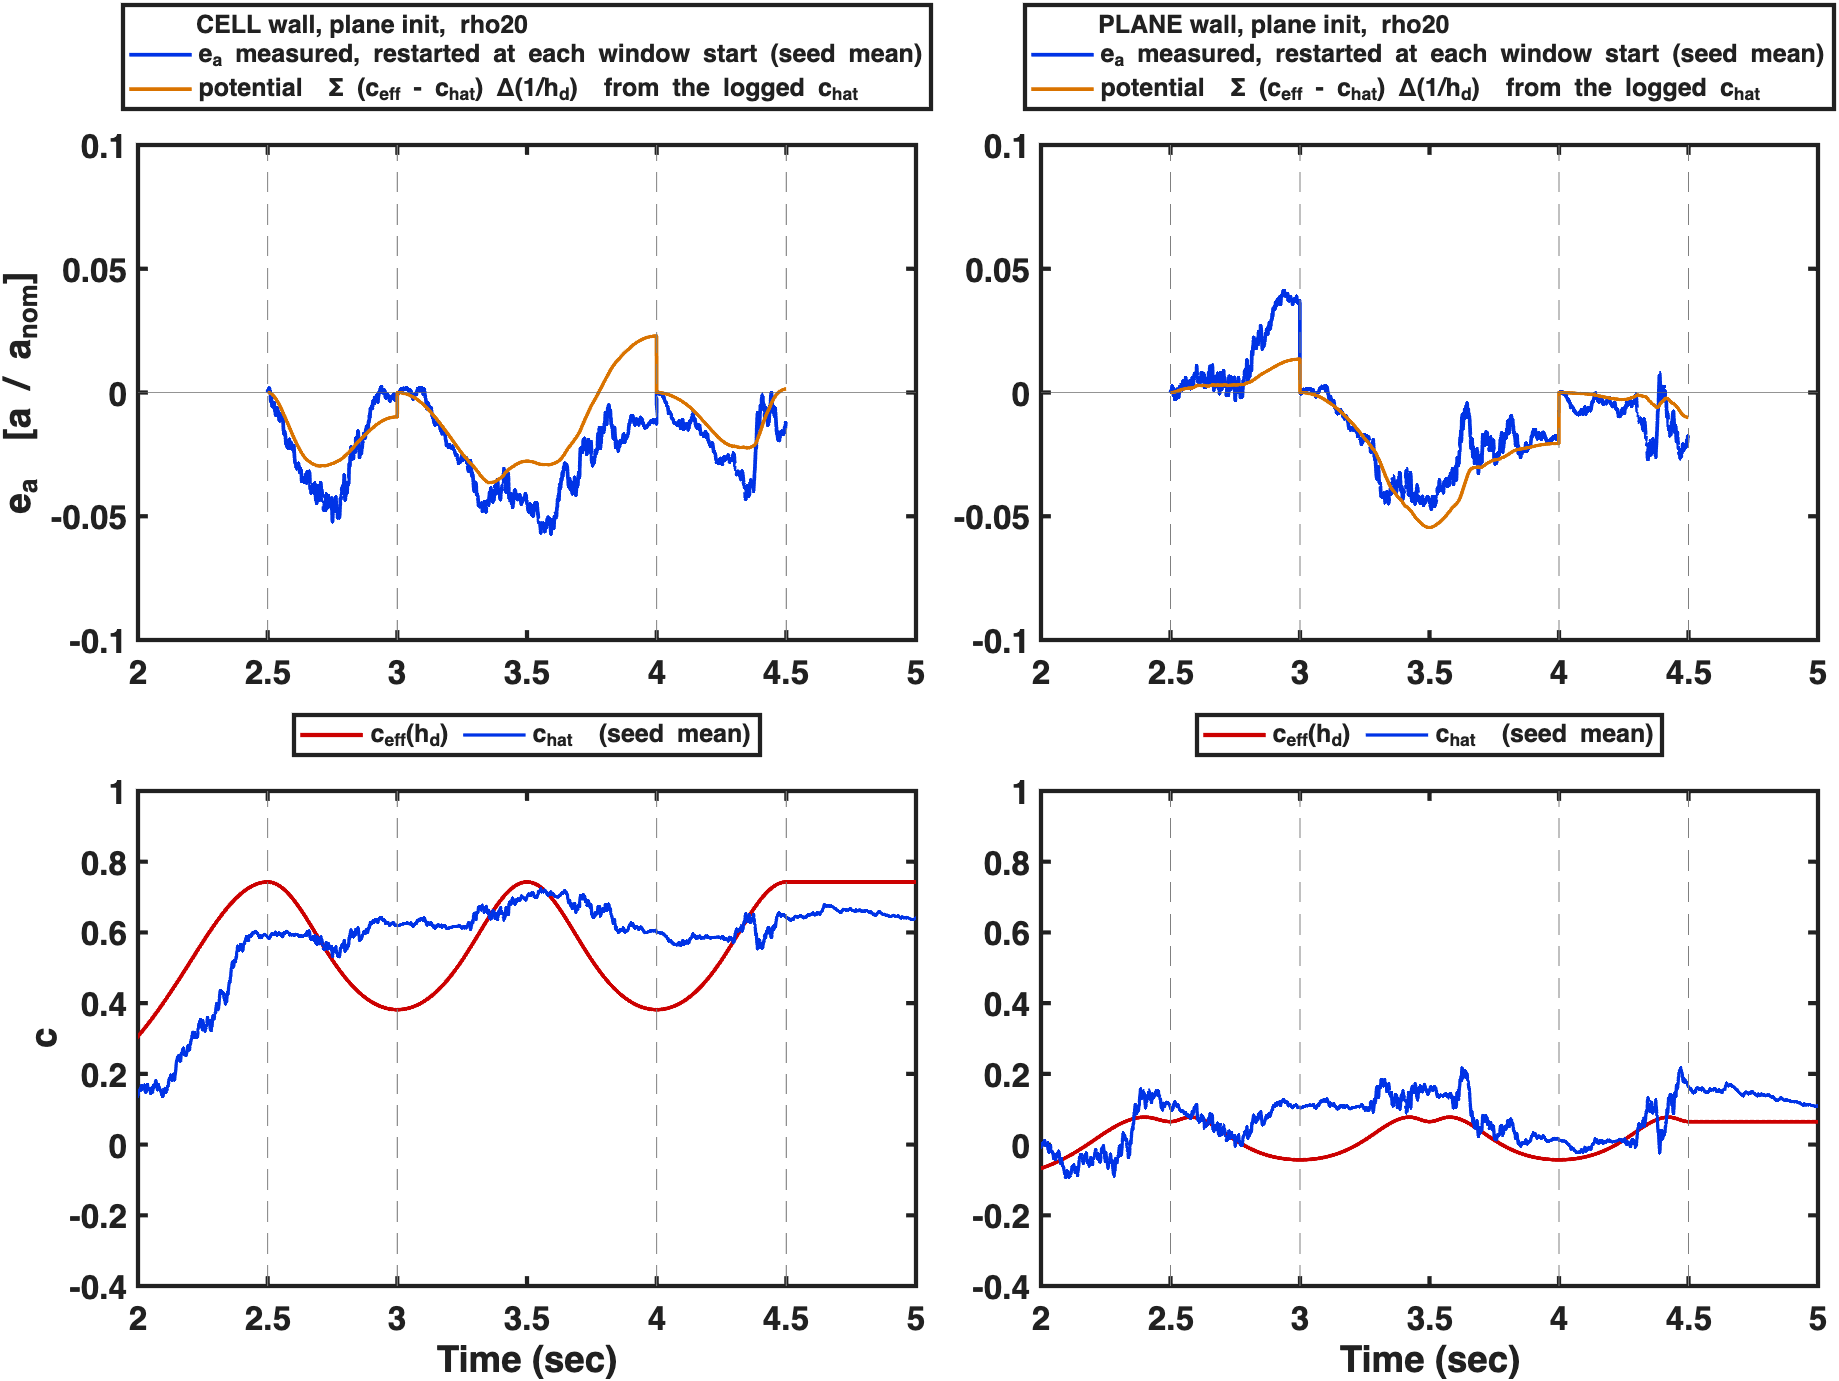
\includegraphics[width=\textwidth,height=0.78\textheight,keepaspectratio]{osc_potential_check_rho20.png}\end{center}

\clearpage
%======================================================================
\section{Cell, ratio $\sqrt{P_0} = 0.2$: ramp 2 s | ramp 2 s + sine 1.10--3.32 R | ramp 2 s + sine 1.05--2.0 R (constant-velocity descent)}
\begin{center}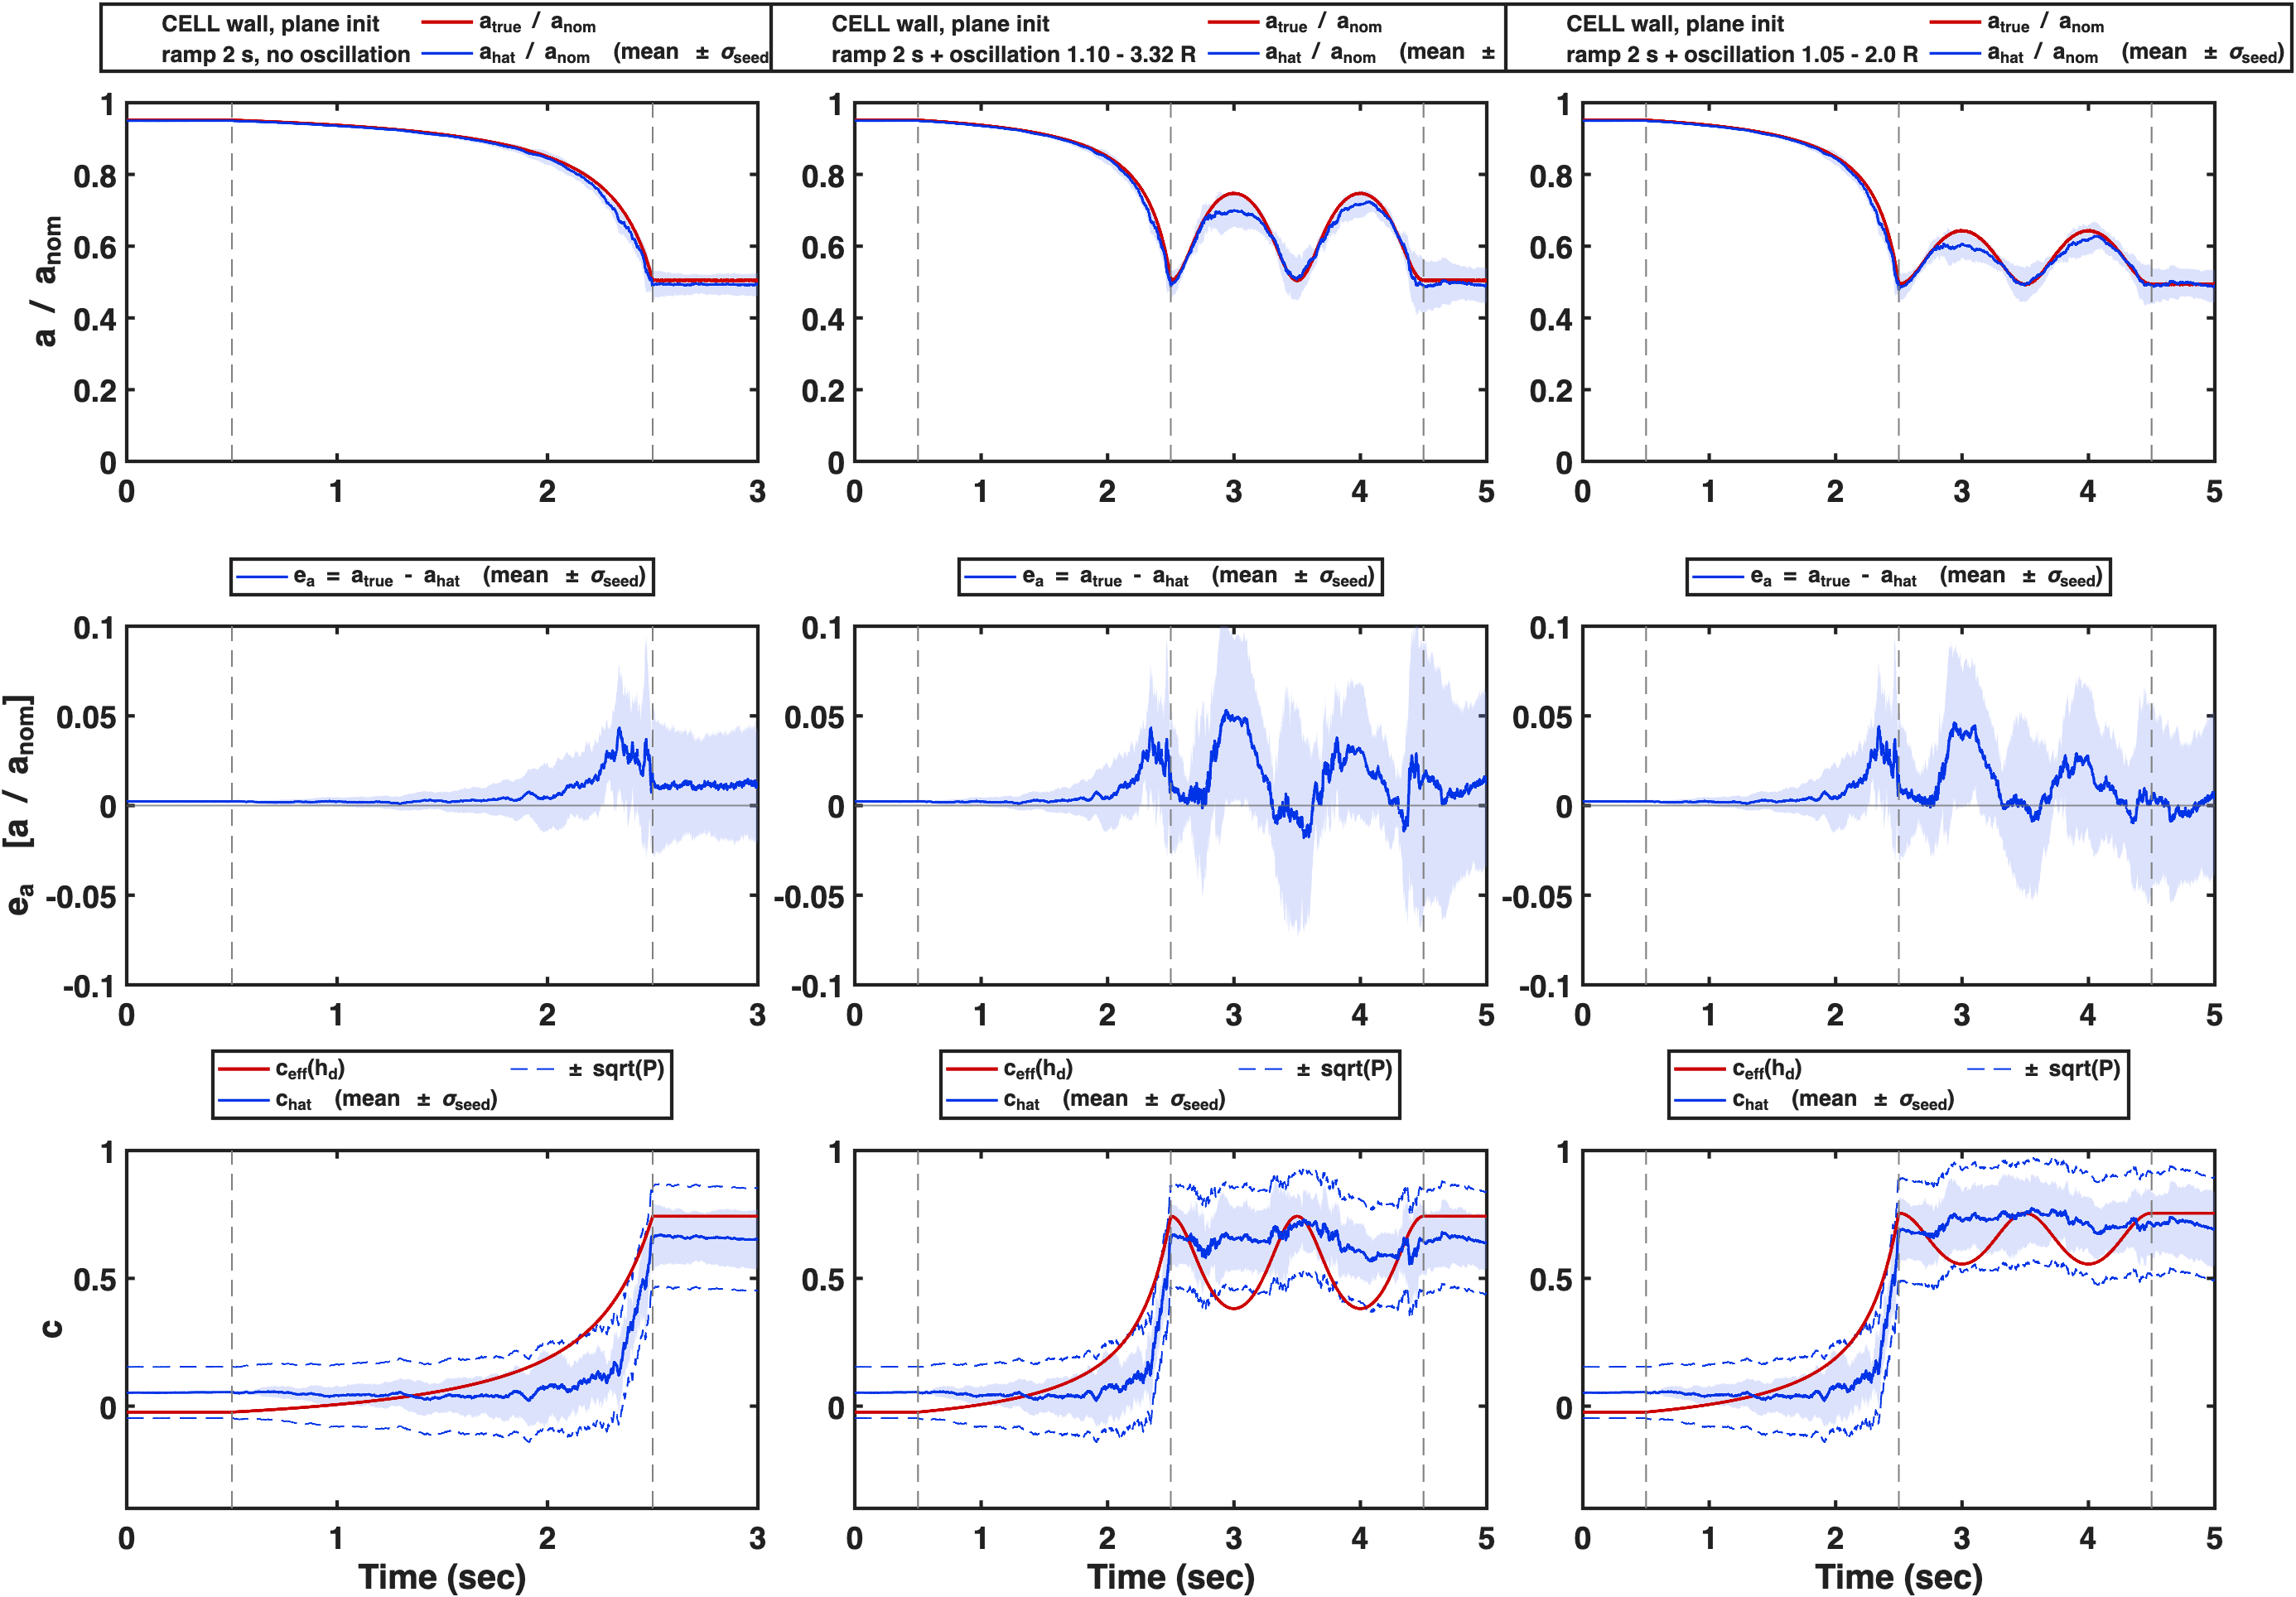
\includegraphics[width=\textwidth,height=0.86\textheight,keepaspectratio]{f1p2_cell_lf_compare_osc_lin.png}\end{center}

\clearpage
%======================================================================
\section{Cell, ratio $\sqrt{P_0} = 0.2$, 0.5 s descent + 1 Hz 1.10--2.0 R: no oscillation | sine | triangle}
\begin{center}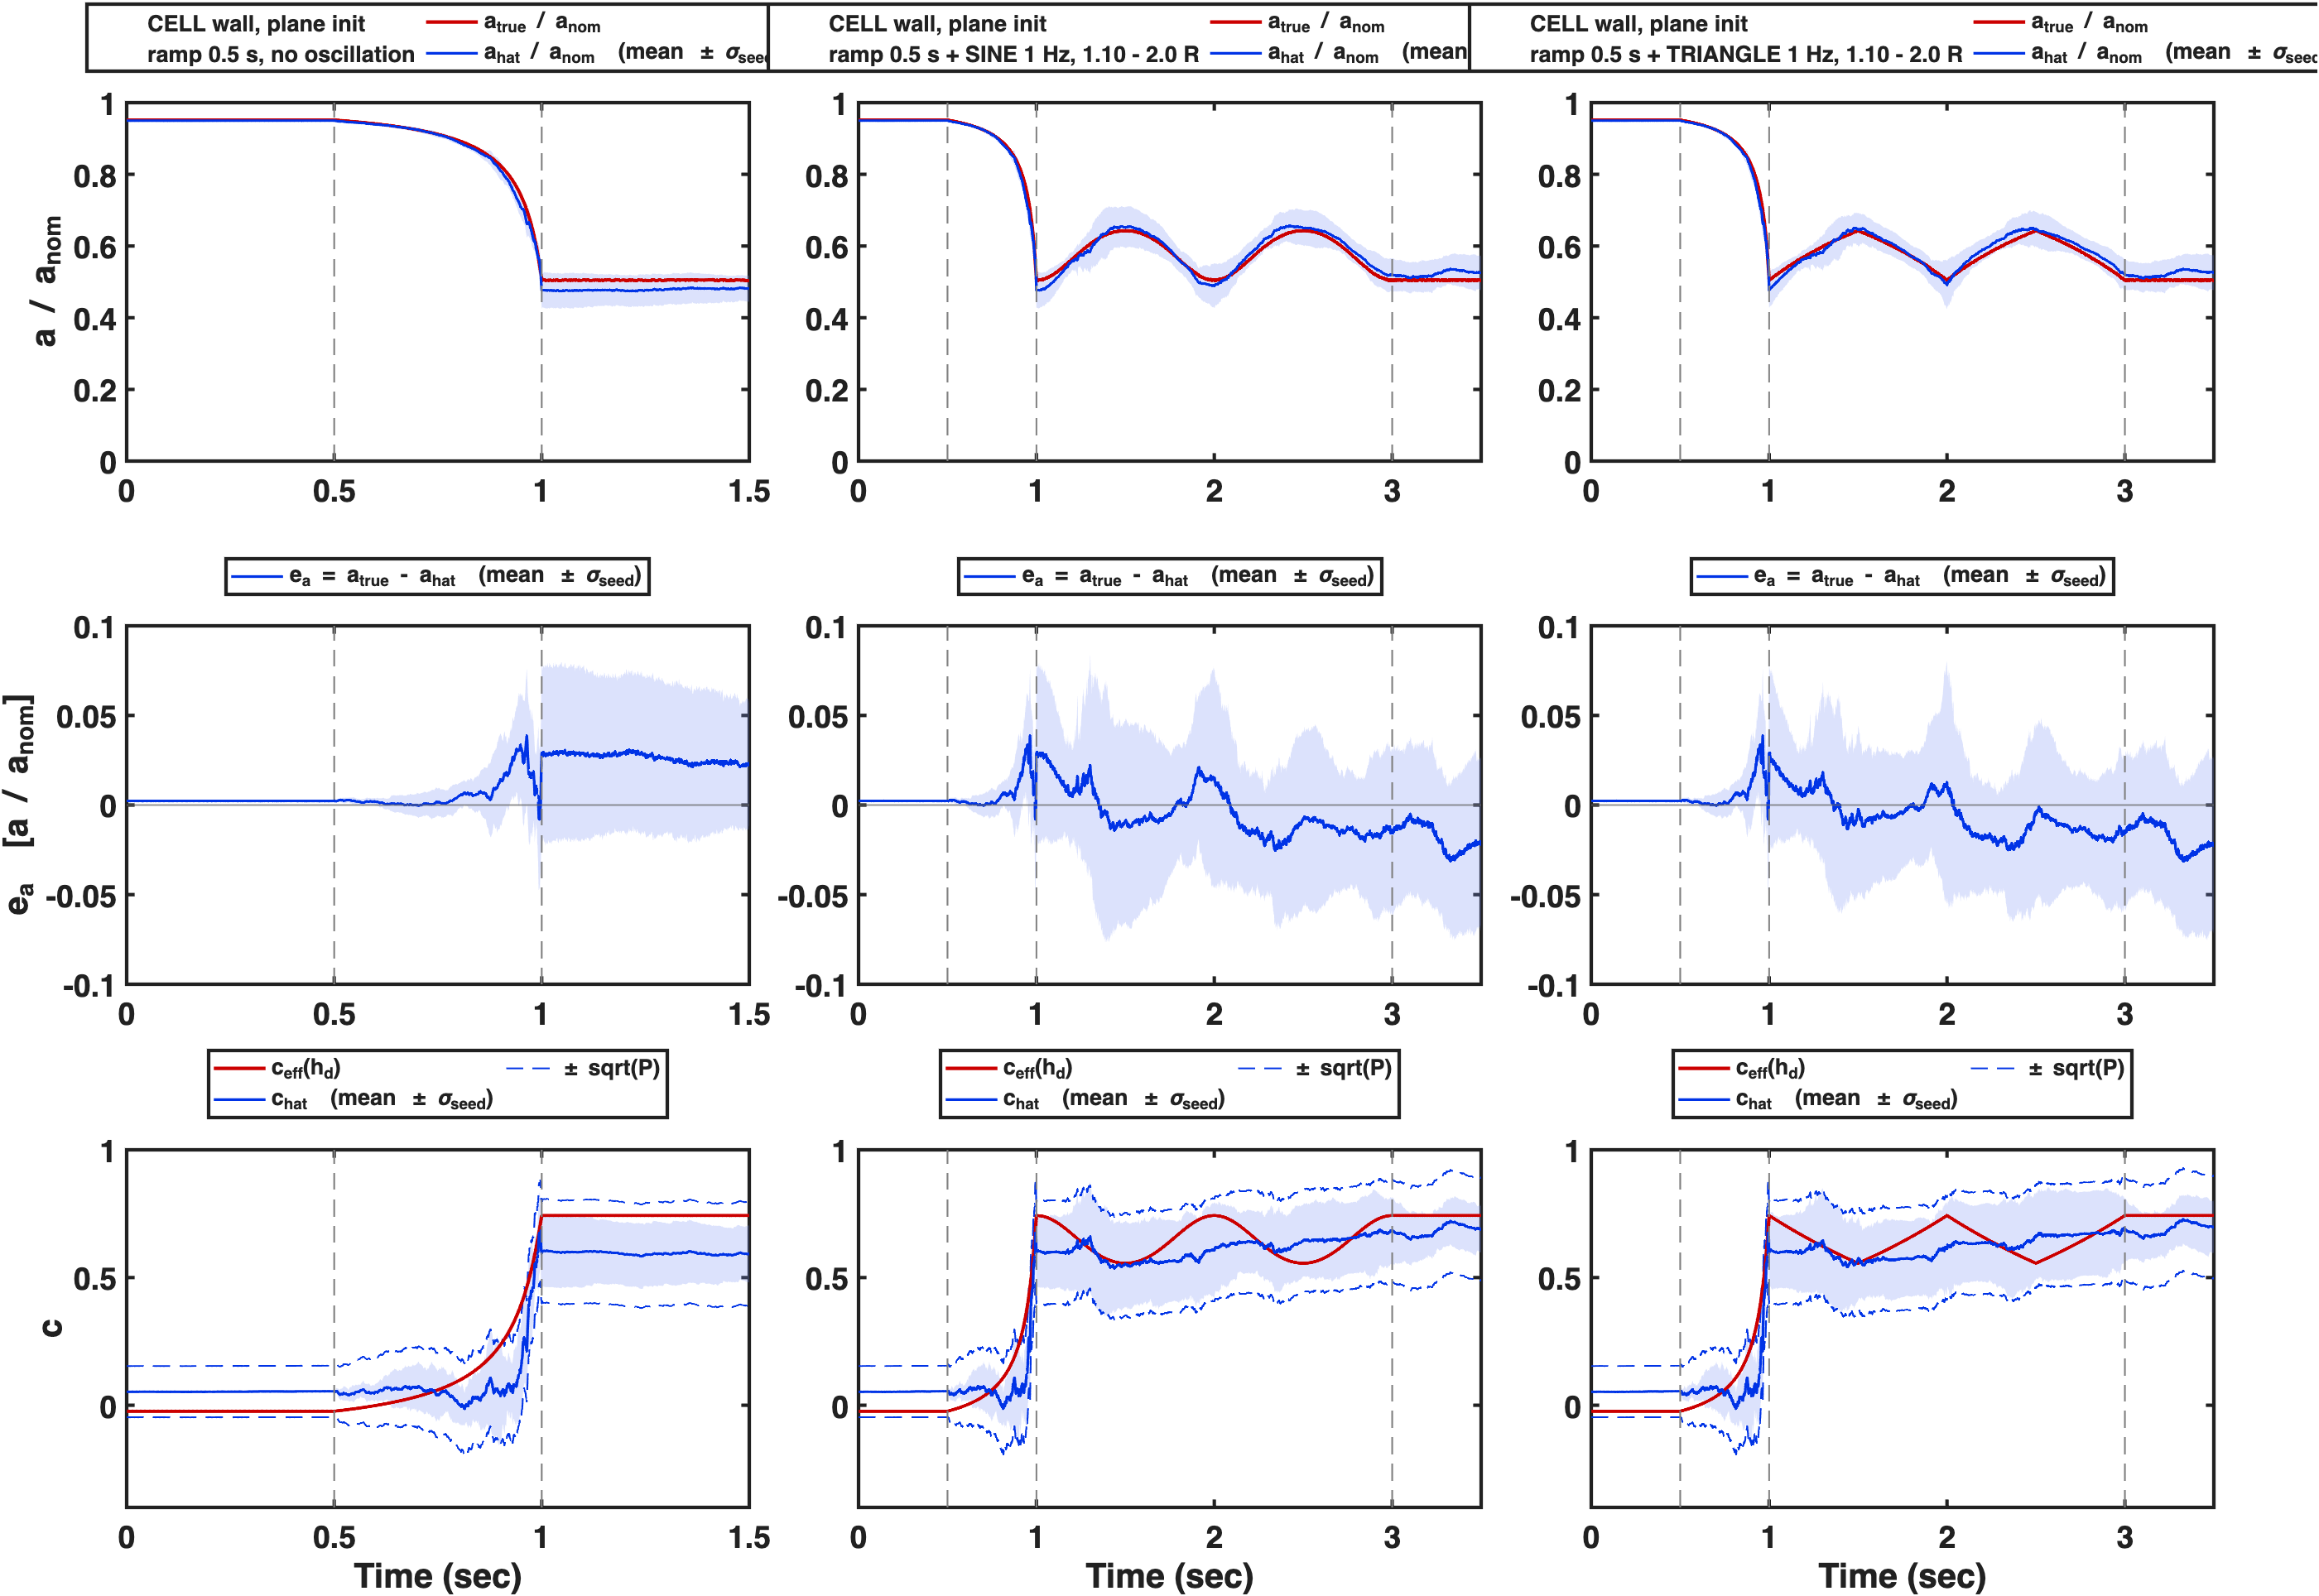
\includegraphics[width=\textwidth,height=0.86\textheight,keepaspectratio]{f1p2_cell_lf_compare_osc_wave.png}\end{center}

\clearpage
%======================================================================
\section{Plane, same three arms (the cost side)}
\begin{center}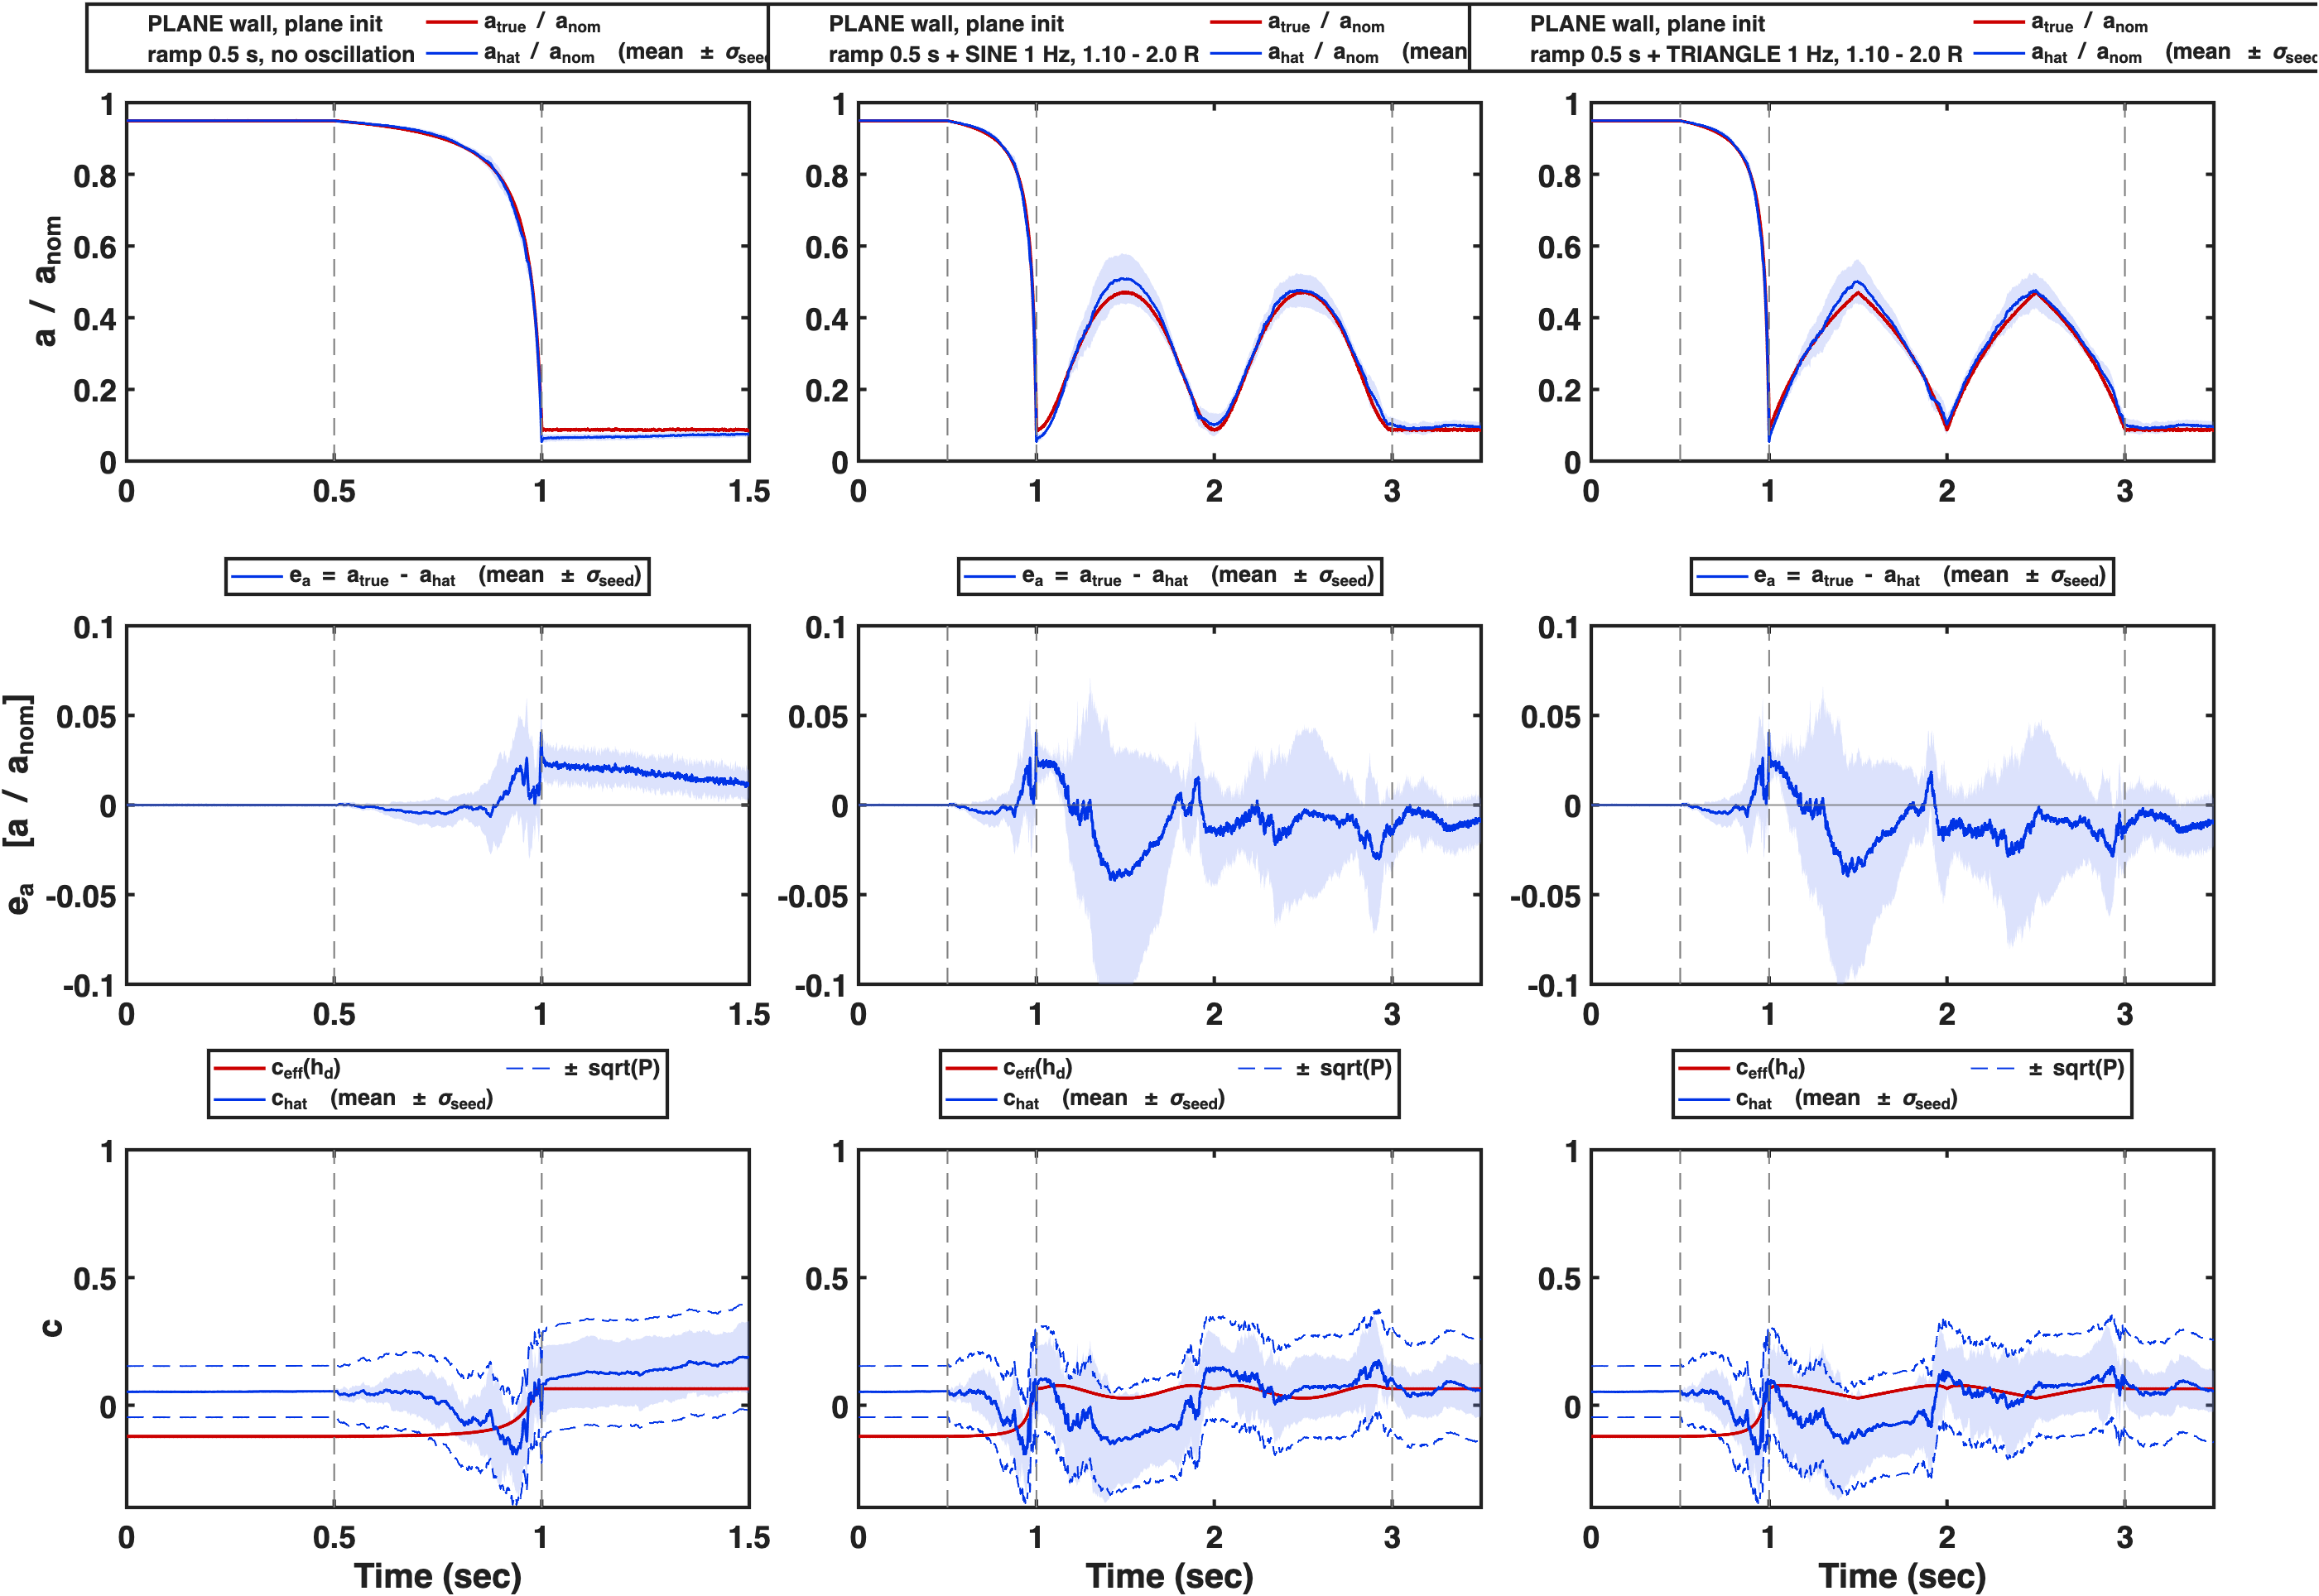
\includegraphics[width=\textwidth,height=0.86\textheight,keepaspectratio]{f1p2_cell_lf_compare_osc_wave_plane.png}\end{center}

\clearpage
%======================================================================
\section{The innovation gate (plane): ratio | ratio $\times$ gate thr 0.2 | thr 0.3}
\[
\nu_1[k] = \frac{\text{innov}_1[k]}{\sqrt{S_1[k]}}, \qquad
s[k] = \frac{1}{100}\sum_{i=0}^{99}\nu_1[k-i], \qquad
Q_{55}[k+1] = P_0^{2}\, I_k\, \mathbb{1}\big[\,|s[k]| > \text{thr}\,\big]
\]
\begin{center}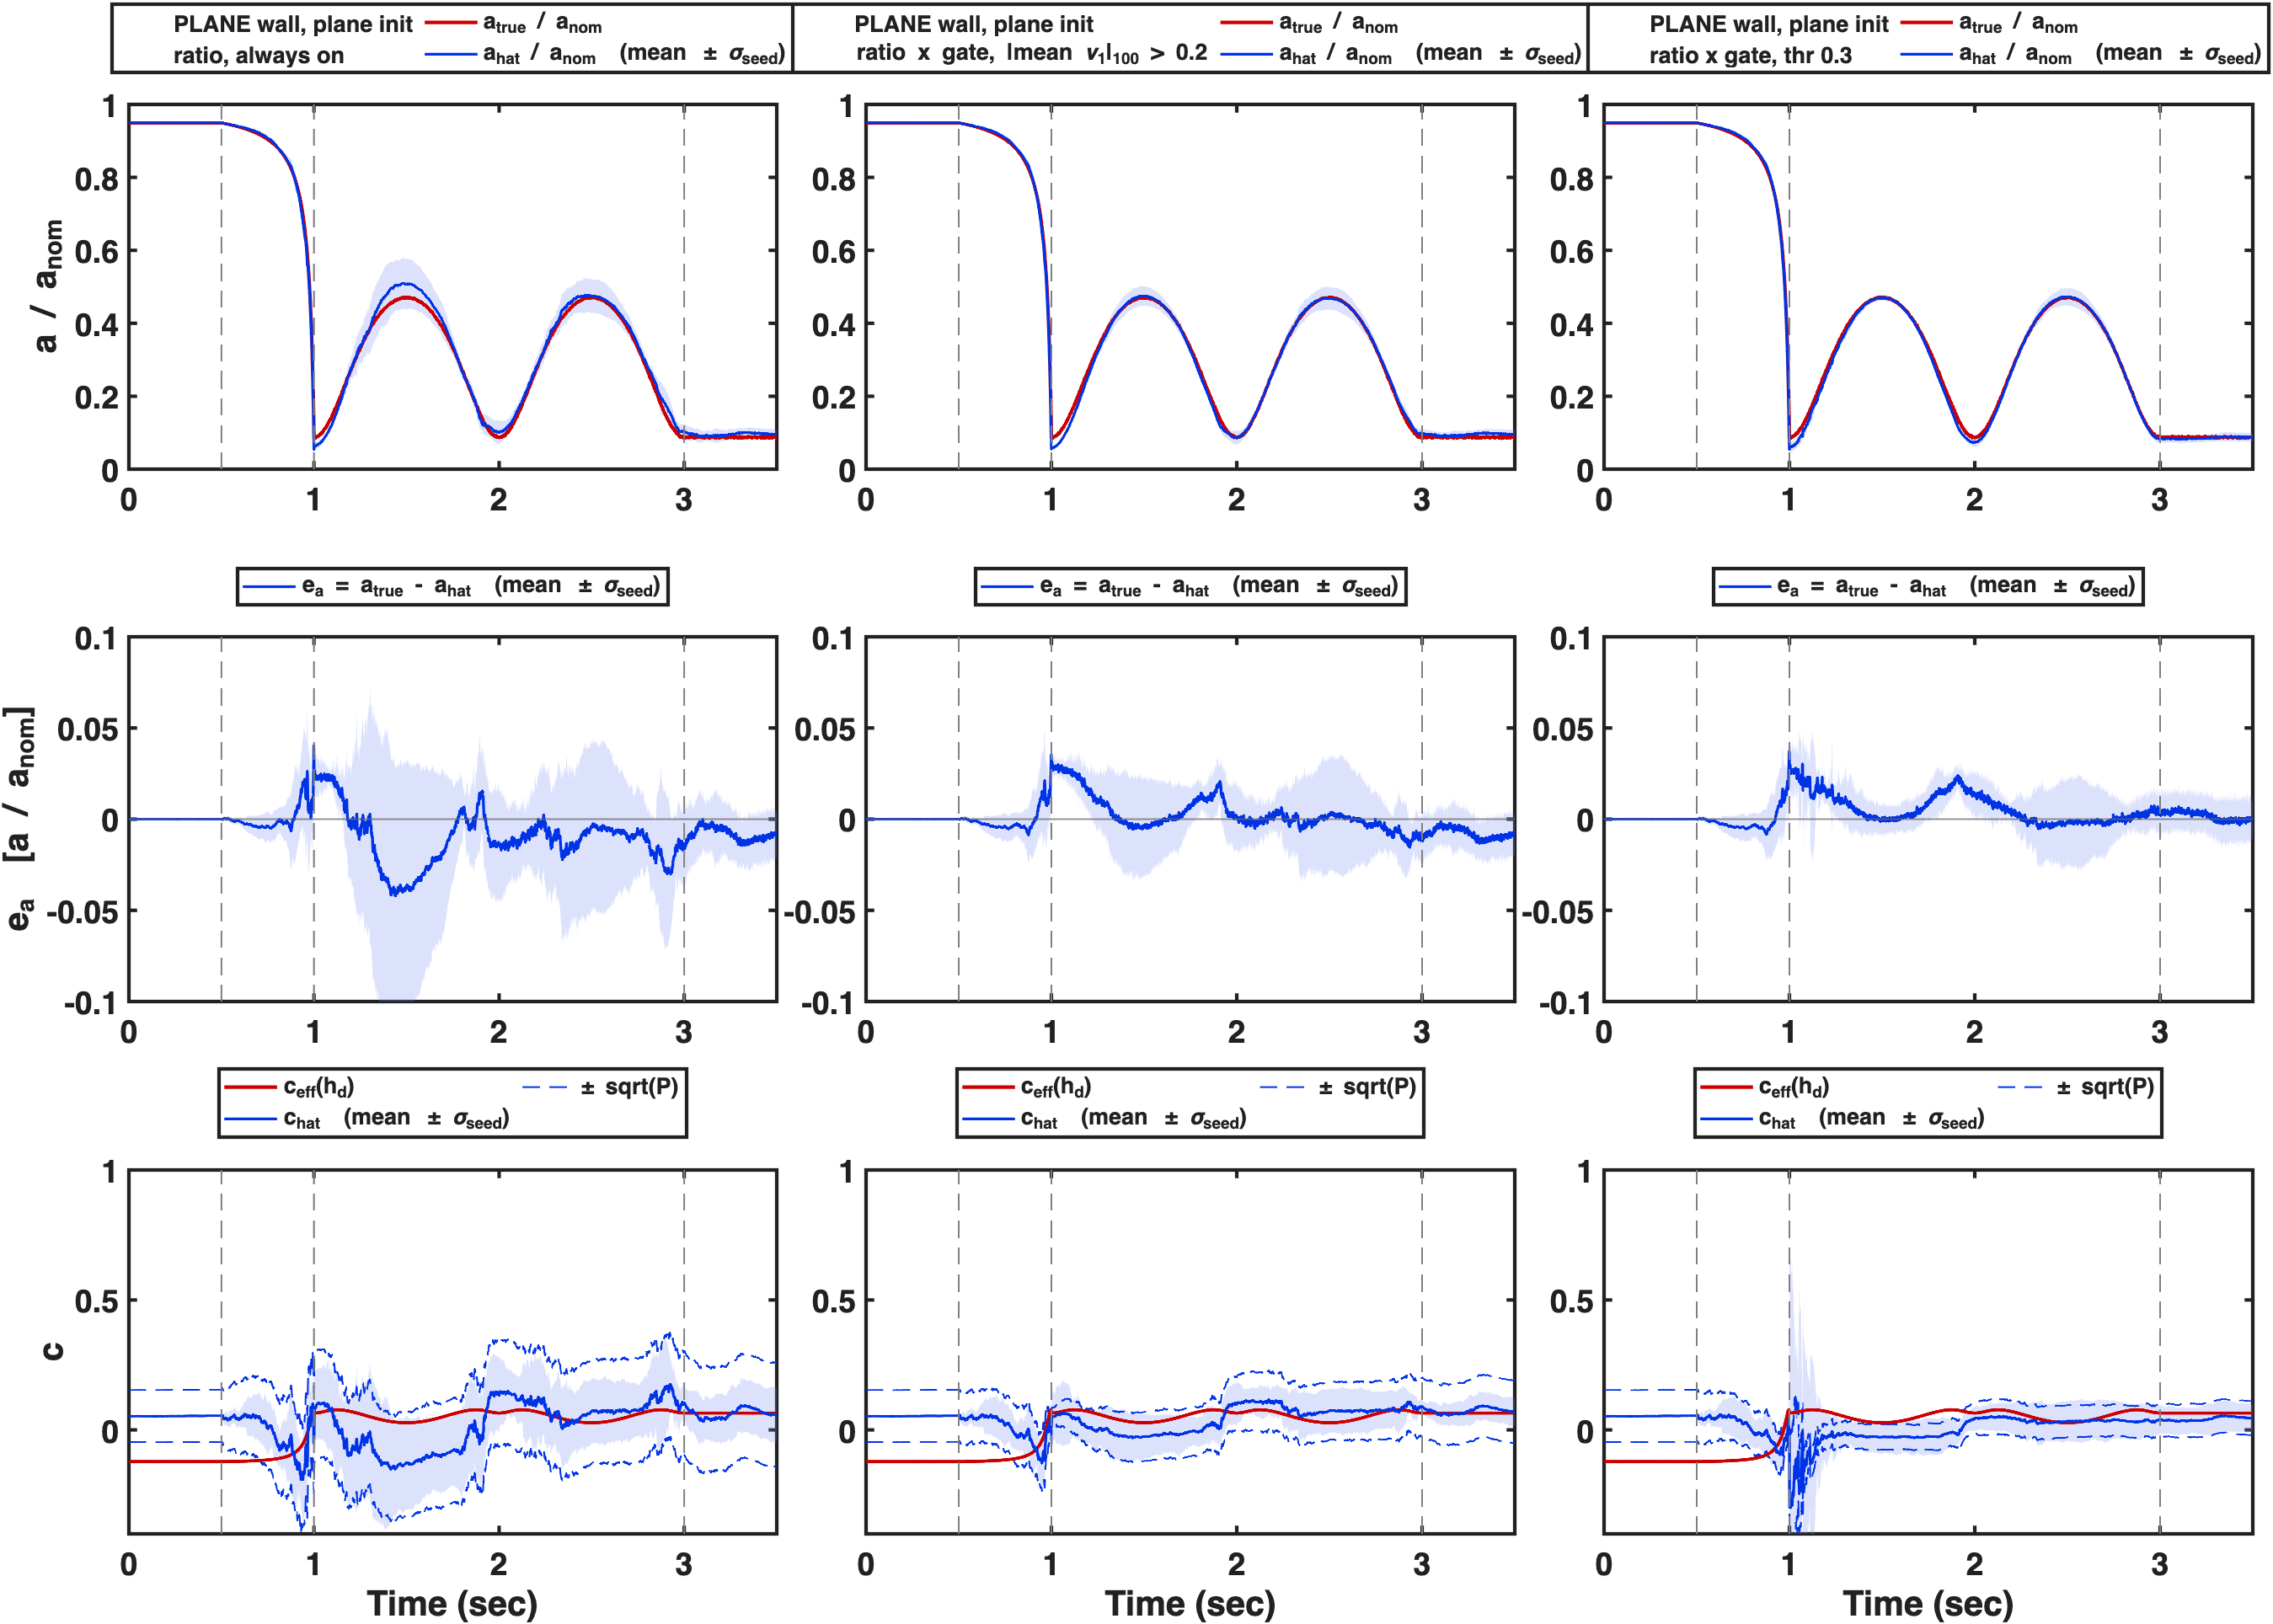
\includegraphics[width=\textwidth,height=0.80\textheight,keepaspectratio]{f1p2_cell_lf_compare_ratiogate_plane.png}\end{center}

\clearpage
%======================================================================
\section{Three designs on one trajectory (cell): ratio | ratio $\times$ gate | constant $R_2$ ratio}
\begin{center}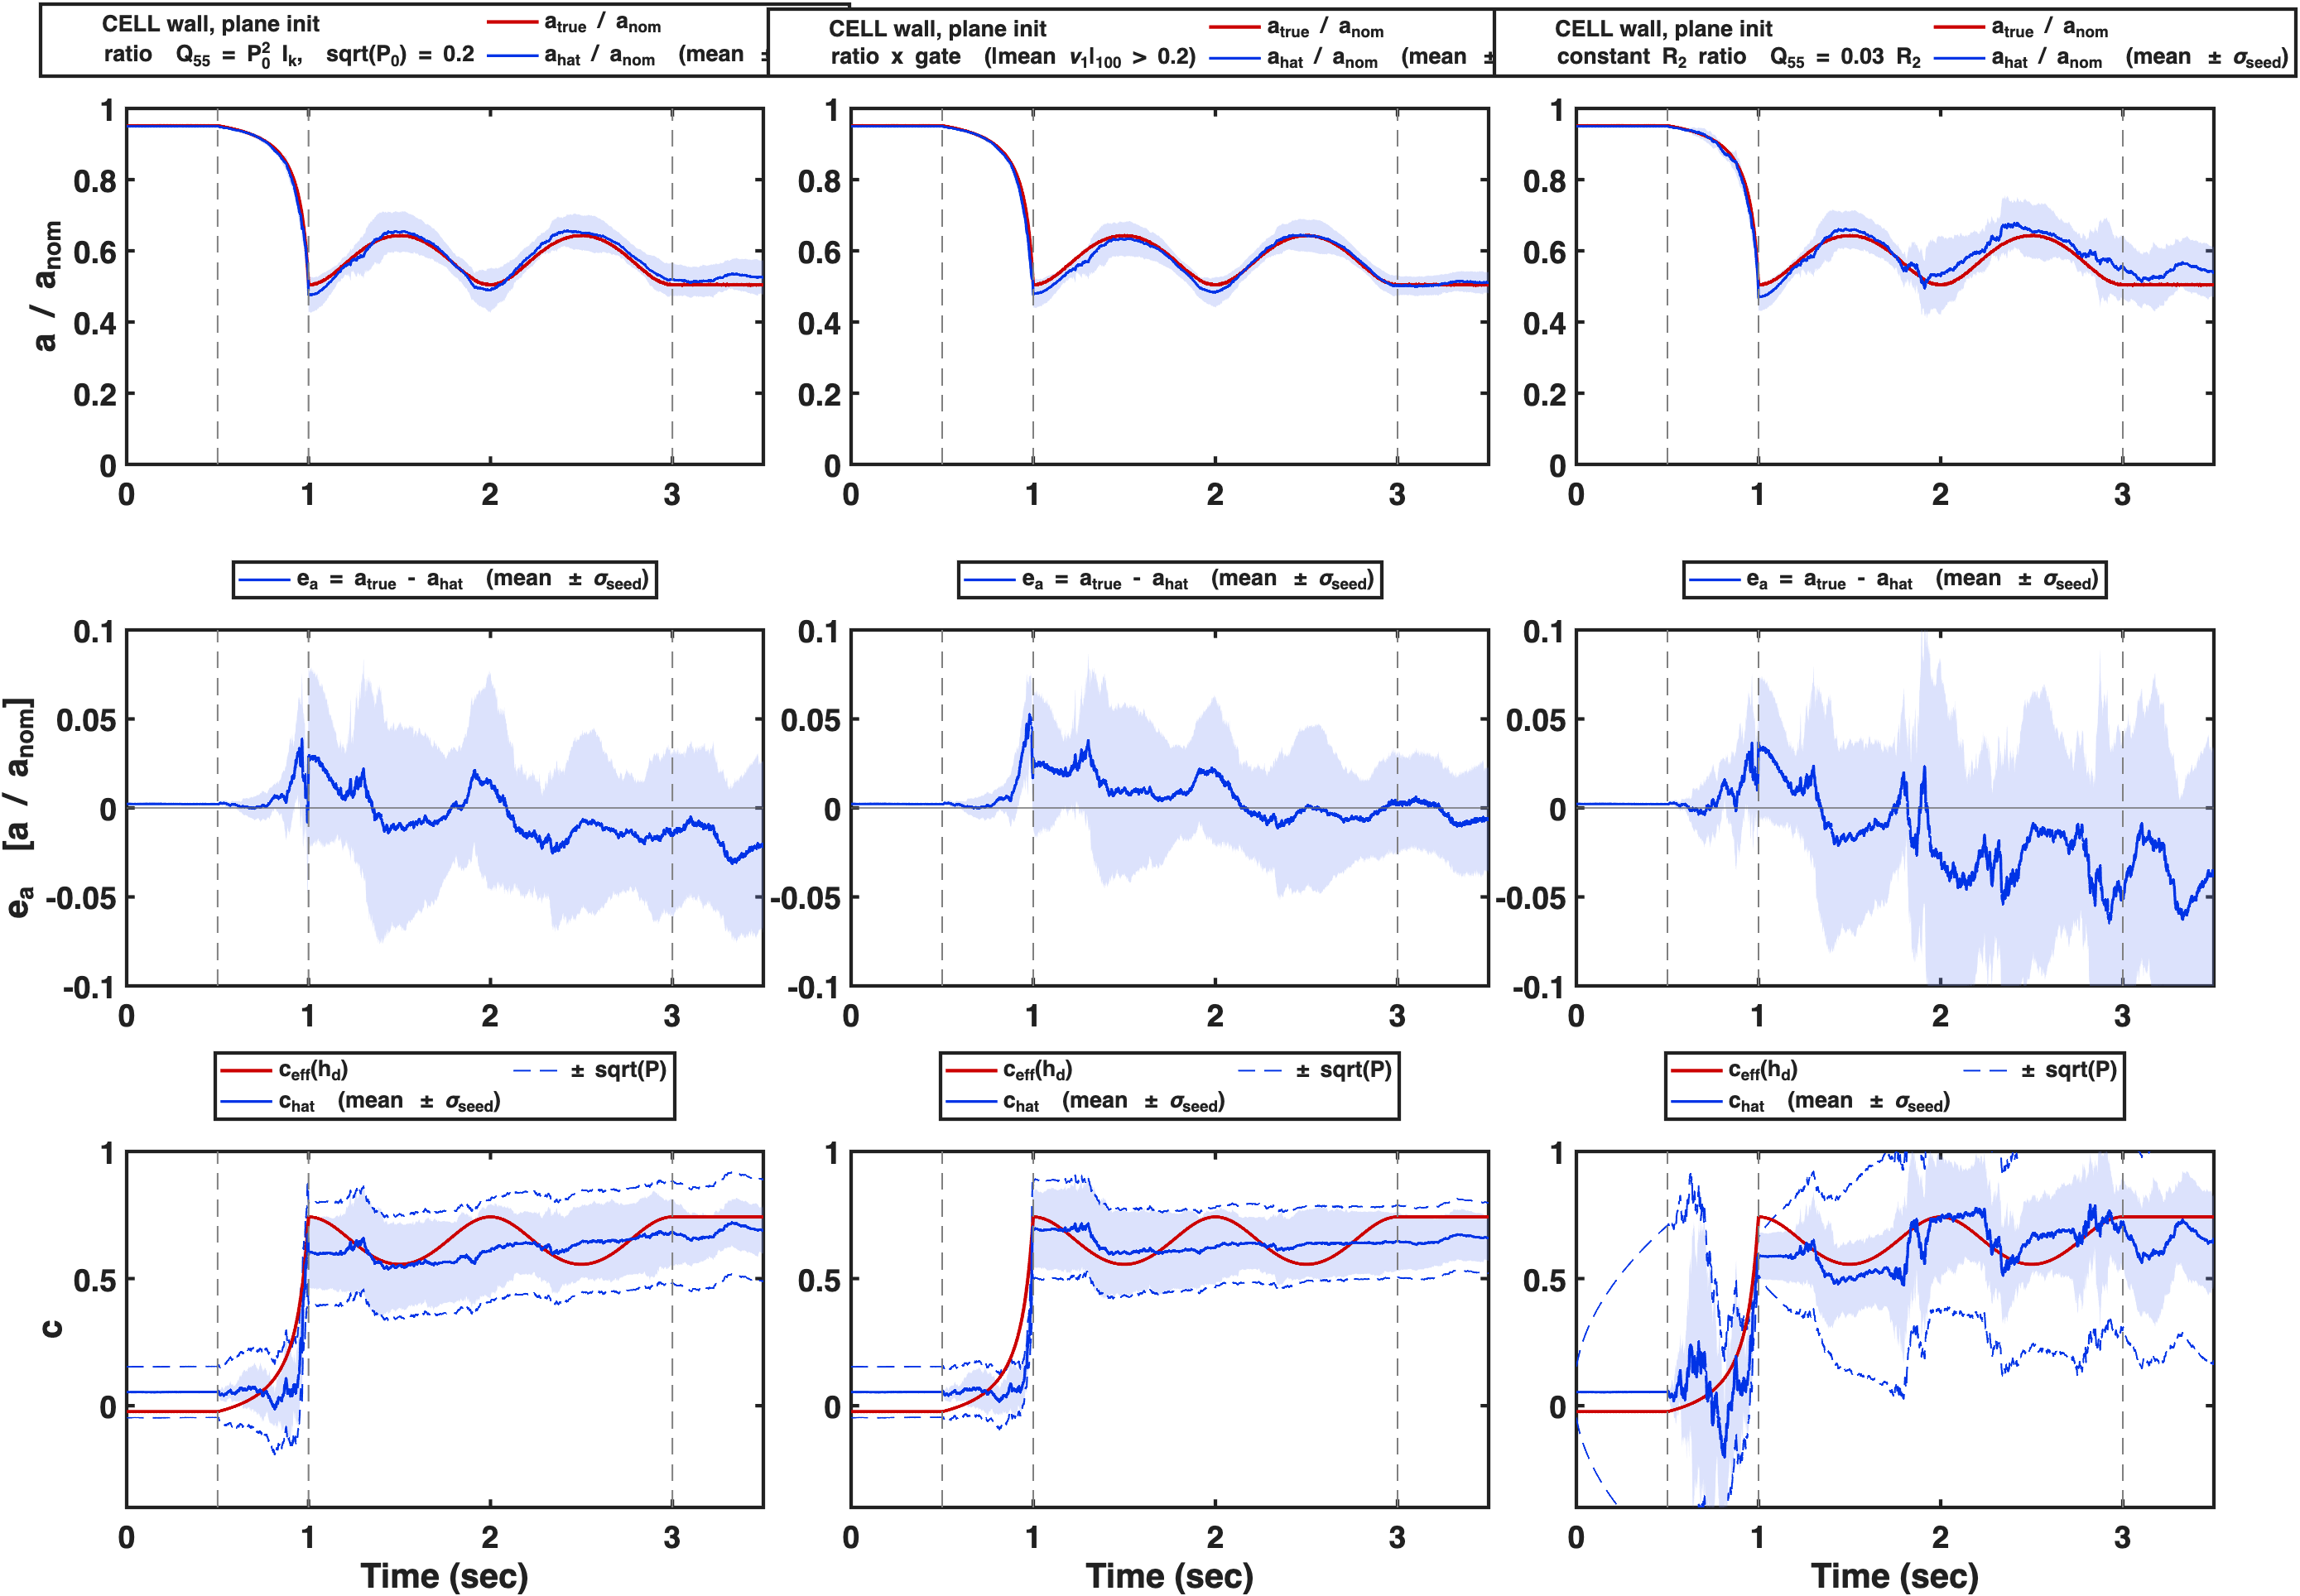
\includegraphics[width=\textwidth,height=0.86\textheight,keepaspectratio]{f1p2_cell_lf_compare_three.png}\end{center}

\end{document}
